\documentclass[b5paper,10pt,dvips,fleqn,titlepage,twoside]{book}
%\pagestyle{headings}
\usepackage[utf8]{inputenc}
\usepackage{amsfonts}
\usepackage{verbatim} 
\usepackage{fancybox}
\usepackage{url}
\usepackage{listings}
\lstset{language=C}
\usepackage[ngerman]{babel}
\usepackage[T1]{fontenc}
\pagestyle{headings}
\usepackage{rotating}
\usepackage{subfigure}


\usepackage[dvips]{hyperref}
\hypersetup{%
   pdfauthor=Michael Durrer,%
   pdfstartview=%
}

\author{Michael Durrer}
\title{Linux Game Development}
\usepackage{makeidx}
\makeindex
\begin{document}
\begin{titlepage}
\begin{center}
\begin{huge} \textbf{Spiele- und Emulatorentwicklung unter GNU/Linux}\end{huge}
\newline
\large
\textit{Für Anfänger und Fortgeschrittene}
\newline
\begin{small}Geschrieben von \emph{Michael Durrer}, geschrieben mit \LaTeX \newline\end{small}
\medskip
\begin{small}
\begin{description}
\item[Mathematische Grundlagen]{Im Buch gehen wir auch auf mathematische Grundlagen ein, die wir später noch benötigen, wenn es zur Emulator- und 3D-Programmierung kommt. Dieser Teil ist somit quer vernetzt durch das ganze Buch, da sich das gesammelte Wissen sogut wie nur durch ständiges Nachschlagen erarbeiten und verwenden lässt.}
 \item[Computer]{Mit einfachen und verständlichen Einführungen in die verschiedenen Computer-Architekturen von früher und heute sowie einem Ausblick in die Zukunft gehen wir dem Begriff \textbf{Computer} auf die Spur und ergründen, wie sich ein Computer definiert und wozu er dient.\newline Ausserdem betrachten wir verschiedene Anwendungszwecke und Historisches.}
\item[Programmierung]{Mittels mehrer Programmiersprachen wie \textbf{C/C++} und \textbf{Python} führt der Autor leichtverständlich in die Tiefen der Programmierung.
Jede der obig genannten Programmiersprachen wird ausreichend gewürdigt und werden mit der Themenpalette des ganzen Buches verknüft. Nicht zuletzte deswegen ist dies der umfangreichste Teil des Buches.}
\item[Linux]{Linux und seinen Derivaten gebührt eine blühende Zukunft. Zwar ist dieser profane Grund nicht der einzige um den Schwerpunkt dieses Buches hierrauf legen zu lassen, doch gibt es im Buch zahlreiche Erläuterungen zu den bekannten Lizenzen und deren Wesen. Auch eine Einführung in Linux darf natürlich hier nicht fehlen; quer vernetzt mit den anderen Themata ergiebt sich hier das ideale Nachschlagebuch für Anfägner wie Fortgeschrittene.}
\item[Emulation]{Durch die vernetzten Kapitel in diesem Buch sind fast überall Referenzen zur Emulation. Dabei gehen wir auf Basiswissen ein mit dem Ziel, am Schluss selber einen eigenen Emulator entwickeln zu können.}
\item[Netzwerk]{Durch der heutzutage überall anzutreffenden Netzwerkfähigkeit wird auch hier ein scharfes Auge hineingeworfen. Wir schauen alle Strukturen, Konzepte und Einsatzgebiete an.}
\item[Multimedia]{Im Zeitaler zahlreicher Medien, ist es wichtiger denn je, ein Verständnis dafür zu entwickeln. Das Hauptaugenmerk liegt in diesem Buch dem optischen Part: Farbenlehre bis generelle Grafik-/Spiele-/Emulatorprogrammierung, so dass auch nicht andere Multimediagebiete wie Audio zu kurz kommen.}
\end{description}

\end{small}

\end{center}
\bigskip


\footnotetext{ Last update on \today }
\end{titlepage}
\newpage
\tableofcontents
\setcounter{secnumdepth}{2}
\part{Einleitung}
\chapter{Vorwort}
Sie haben dieses Buch gekauft, von meiner Seite als PDF heruntergeladen oder über andere Wege erhalten, mit einem bestimmten Hintergedanken und einer Erwartungshaltung. Und vielleicht haben Sie sich auch schon einmal eine der folgenden Fragen an den Kopf geworfen:

\begin{flushleft}
\emph{
Wie programmiere ich ein Spiel, einen Emulator oder eine beliebige Anwendung \underline{f\"{u}r Linux?}\newline Wo(mit) fange ich \"{u}berhaupt an?\newline Kann ich das überhaupt?}\newline
Was benötige ich dazu?\newline Was ist möglich?\newline
\end{flushleft}

So ähnlich zumindest waren meine (zahlreichen) \"{U}berlegungen, als ich vor vielen Jahren angefangen habe, mich mit der Interna von Rechnern und der Digitaltechnik herumzuschlagen. Seien Sie also nicht beunruhigt, jeder ist sich anfangs unsicher. Und in Erinnerung an die Problematik dieses Beginns (der heute in der riesigen F\"{ü}lle an Informationen im Internet immerhin erleichtert worden ist), m\"{o}chte ich dieses Buch all denen zur Verf\"{u}gung stellen, die sich gerade inmitten jener Phase befinden und händeringend brauchbare Informationen suchen oder bereits diverse Grundlagen besitzen und darauf aufbauen m\"{o}chten.\newline
Vielleicht haben Sie bereits früher einmal versucht ein Spiel zu programmieren und es gelang Ihnen nicht, die Applikation fertigzustellen (übrigens eine der häufigsten Ursachen für den Abbruch eines Projektes: \textit{Motivationsverlust}). Möglicherweise sind Sie auch schlichtweg an einer Stelle in Ihrem Workflow angeeckt und haben keine Lösung für das Problem gefunden.
Gerade in solchen Fällen ist es mein Ziel, Ihnen mit diesem Buch lückenlos jede Stufe der praktischen Umsetzung von der Idee zur Applikation aufzuzeigen oder zumindest als Stütze dienen zu können.
Aus den verschiedenen Beweggründen und Ursachen, die jemanden zu diesem Buch geführt haben, lassen sich verschiedene Typen herauskristallisieren und auf einen gemeinsamen Nenner bringen: So mögen Einige bereits programmieren können in C/C++, Andere haben gar noch nie etwas entwickelt aber würden gerne den Einstieg finden und wieder Andere wollen sich schlichtweg weiterbilden, zum Beispiel über SDL und Emulatoren. Aus diesem Grund habe ich dieses Buch in mehrere Parts unterteilt, welche sich an verschiedene Niveaustufen richten und Neueinsteigern wie Quereinsteigern einen Einstieg in die Thematik bieten kann. Diese Parts sind:
\newline

\begin{itemize}
\item Einleitung
\item Computer und Mathematik
\item GNU Linux - Das fremde System
\item Versionsverwaltung mit Subversion
\item Programmieren mit Python
\item ANSI-C-Kurs für Anfänger
\item C++ Kurs (aufbauend auf den ANSI-C Kurs)
\item Grundlagen der Netzwerkprogrammierung
\item Die Grundlagen von Python
\item SDL - Der Simple DirectMedia Layer
\item Emulation - Fremde Systeme simulieren
\end{itemize}\medskip
Dabei ist der Schwerpunkt auf Linux gesetzt, doch habe ich auch durchgehend Wert auf Portabilit\"{a}t gelegt. Alle Programmbeispiele sollten auch unter Windows 2000 und höher laufen.\newline
Speziell in der Spielewelt w\"{a}re eine h\"{a}ufigere Verwendung der SDL angebracht, ist sie doch portabel auf alle g\"{a}ngigen Plattformen wie Windows Vista/XP, Linux oder Mac OS X.\newline
Portabel heisst in diesem Sinne, dass durch Verwendung von SDL f\"{u}r Steuer-, Eingabe-, Audio- und Videoger\"{a}te diese universal programmierbar werden. Eine einheitliche API (\textit{Application Programming Interface}) steuert die Ger\"{a}te nun an, der Programmierer sieht nur noch die API und deren Dokumentation. Spezifische Eigenheiten f\"{u}r jeweilige Ger\"{a}te und Betriebssysteme, z.B. verschiedene Grafikkarten, \"{u}bernimmt nun die SDL-Schicht komplett und \"{u}bersetzt sie in die Sprache der jeweiligen Betriebssysteme und Hardware um.\newline

Zus\"{a}tzlich habe ich mich f\"{u}r dieses Buch auf 3 Programmiersprachen festgelegt: \textbf{C, C++ \& Python}.\newline C/C++ ist quasi ein Industrie-Standard und wird seit Jahren in der Applikationsentwicklung da eingesetzt, wo man schnelle und \"{u}bersichtliche Anwendungen ben\"{o}tigt, zu diesen geh\"{o}ren auch grafiklastige Applikationen. Seit einigen Jahren sind aber die Prozessoren mittlerweile an einem Punkt angelangt, wo sich die Entwicklung nicht mehr so stark an Geschwindigkeit multipliziert wie fr\"{u}her.

Die meisten Rechner sind heutzutage schon bei einer Geschwindigkeit angelangt, mit der die meisten Spiele auf dem Markt lauff\"{a}hig sind, zudem wird immer mehr Rechenleistung auf die enorm leistugnsf\"{a}higen Grafikkarten ausgelagert, die auch auf langsameren Rechnern eine gute Grafikleistung hervorzaubern k\"{o}nnen und nicht mehr zwingend eine 'schnelle Programmiersprache' ben\"{o}tigen.

An dieser Stelle springt Python ein: Python ist eine skriptbasierte Sprache, die ebenfalls objektorientiert aufgebaut ist und somit eine exzellente \"{u}bersicht bietet. Desweiteren ist sie sehr einfach zu erlernen und kann ebenfalls mit SDL umgehen, es richtet sich daher eher an die Programmieranf\"{a}nger, was jedoch nicht heissen soll, dass man damit nicht genauso komplexe Applikationen bauen k\"{o}nnte.\newline Wie auch immer Ihre F\"{a}higkeiten und Ihr Wissen derzeit liegen, Ich hoffe Sie finden mit diesem Buch ein Themengebiet, dass Sie weiterbringt und Ihnen einen einfachen Einstieg in die Thematik erm\"{o}glicht.
Beachten Sie jedoch bitte, dass ich Ihnen nahelege, gute Vorkenntnisse in ANSI-C oder C++ mitzubringen, da ich den Grossteil dieses Buches doch darauf st\"{u}tze und auf jeden Fall fr\"{u}her oder sp\"{a}ter f\"{u}r professionelle Anwendungsentwicklung gelernt werden muss.

An den Teil \"{u}ber \textit{Emulation}, sollten sich nur echte Profis ranwagen, welche C/C++ bereits in- und ausw\"{a}ndig kennen. Auch wenn vielleicht nicht alles beim ersten Durchlesen verst\"{a}ndlich sein mag f\"{u}r Anf\"{a}nger, interessant ist es dennoch auf alle Fälle. Gleichzeiti wird Fach- und Hintergrundwissen vermittelt, welches unterstützend mitwirken kann beim Verst\"{a}ndnis Abläufe in der Programmierung.
Denn nur wer genau versteht, was sein Gerät spricht und tut, kann ihm genau befehligen, was und wie das Gerät es zu tun hat.

Einen Schwerpunkt habe ich beim Schreiben des Codes auf Übersichtlichkeit und einfachen Code, für Anfänger verständlich, gelegt, da es mir sehr wichtig war, Anfängern bereits die Möglichkeit zu bieten, komplexere Vorgänge wie Video- und Audioprogrammierung zwar nicht zwingend selber programmieren zu können, doch zumindest das Prinzip zu verstehen.

Neben dieser geballten Ladung an Information und Wissen, dass Sie in gebundener Form vor sich liegen haben, sollten Sie jedoch ein Punkt nie aus den Augen verlieren: Programmieren ist nicht nur lernen und arbeiten, sondern bereitet auch durchaus Entspannung und Spass! Und eben diese w\"{u}nsche ich Ihnen nun mit diesem Buch und entlasse Sie hiermit in die spannende Welt der Linuxprogrammierung...


Ihr Michael Durrer
\newpage
\part{GNU Linux - Das fremde System}

\chapter{Linux - Was ist das eigentlich?}
\section{Eine kleine Einleitung}
Bestimmt haben Sie schon einmal von \emph{Linux} gehört oder vielleicht sogar Erfahrungen damit gesammelt. Von einem Nischensystem mit zweifelhaftem Ruf hat es sich zu einer ernstzunehmenden Software entwickelt, die kommerziellen Betriebssystemen wie \emph{Windows XP} oder \emph{Windows 2003 Server} in jeder Hinsicht  Paroli bieten kann.\newline Dabei wird es vorwiegend im Server-Bereich eingesetzt da es durch seine hohe Transparenz und Stabilität bei gleichzeitig hoher Leistung hervorsticht. Beachtenswert ist hierbei vorallem, dass Linux dadurch, dass es in \emph{C} geschrieben wurde, hochportabel ist. Sprich: Es lässt sich auf nahezu jede beliebige Platform umsetzen, die über einen \emph{ANSI-C kompatiblen Compiler}\footnote{Ein Compiler übersetzt Quelltext (\textit{engl. Source-Code} in ausführbare, binäre Dateien/Programme.} verfügt und über einige Megahertz und ein paar Megabyte Arbeitsspeicher verfügt.\newline
Um es jedoch einmal technisch auszudrücken: \textbf{Linux} oder \textbf{GNU/Linux} ist ein freies Multiuser-Betriebssystem, welches strukturell auf Unix basiert, jedoch komplett auf einen eigenen Source Code aufbaut. Beachten muss man dabei, dass wir hier nicht wie zum Beispiel bei Windows einfach \emph{ein Linux} gibt, sondern Linux schlichtweg nur der Kern (auch Kernel genannt), der Hauptbestandteil. Dann gibt es dann noch die \emph{Distributionen}, das sind dann die eigentlichen Systeme; Software-Zusammenstellungen für verschiedene Anwendergruppen. Die Entwicklung des Systems wird weltweit von meist privaten Software-Entwicklern geleitet, die an verschiedenen Projekten arbeiten und so einen gigantischen Software-Pool für Linux aufbauen und natürlich eben auch am Kern selber mitentwickeln.
\newline
Der Kernel steuert die komplette Hardware, er beinhaltet Treiber und ist modular aufgebaut, so dass man jederzeit Module (= Treiber/Erweiterungen) selber nachladen oder entfernen kann. Durch die gute Dokumentation und den offenen Quelltext der Software kann jede beliebige Person eine eigene Version eines Programmes entwickeln oder auch seine Änderungen in das Projekt miteinfliessen lassen, insofern der Projektverwalter-/verantwortliche, den Code geprüft und gestattet hat.
\section{Herkunft}
Linux hat seine Wurzeln in Finnland im Jahre 1991 beim Entwickler \textbf{Linus Torvalds}, damals noch Student, als er begann, ein Unix-ähnliches Betriebssystem zu entwickeln. Er kündigte dies im \emph{Usenet} an, dass er es bald zur Verfügung stellen werde für Interessierte. Bald darauf gab er ihm, inspiriert durch den Administrator des Servers, wo er das System gelagert hatte, in Anspielung auf seinen Namen, Linux.
Damals stand es noch unter einer eigenen Lizenz, die eine kommerzielle Nutzung komplett ausschloss, jedoch bemerkte Torvalds, dass dies für die Weiterentwicklung des Systems hinderlich war und hob diese Begrenzung auf und entschied sich mit den mittlerweile hinzugekommenen Mitautoren, das System unter die \emph{GNU GPL} zu stellen. So geriet Linux in das GNU-Projekt und dieses hatte nun eine Basis, denn das Ziel des GNU-Projektes war es, eine freie, d.h. eine für jeden gratis und offen verfügbare Version von Unix zu entwickeln. Durch diesen Schritt wurde Linux für eine immer grössere Anzahl an Entwicklern interessanter, was sich durch die grosse Bereitschaft zeigte, mitzuhelfen; der Quelltext vergrösserte sich rasant und Linux vebreitete sich bei Hobby-Entwicklern aber auch speziell in studentischen Kreisen.
\newline
Die damals durch den rasanten, ungeplanten Aufstieg des Betriebssystemes, etwas chaotische Arbeitsweise, führte zunächst zu einem wenig übersichtlichen Quelltext, so dass es viele Überarbeitungen gab und zuletzt mit dem Versionsschritt von 2.4 auf 2.6 endgültig ein Schritt in eine modernere, übersichtlichere Richtung getätigt wurde, die nun eine grosse Anzahl an moderner Hard- und Software unterstützt. Die Organisation ist heute klar strukturiert und die Zulassungen für strukturelle Änderungen am Kernel liegen immer noch unter der Obhut von Linus Torvalds.\\
\newline
Jedoch kann man, wie schon erwähnt, durch die GPL eine eigene Version von Linux entwickeln und sich nach seinen eigenen Wünschen gestalten, falls einem die Richtung der offiziellen Entwicklung nicht gefällt oder man spezielle Vorhaben hat. Letzten Endes können diese Erweiterungen und Anpassungen auch womöglich wieder zurück in den Kernel fliessen und so der ganzen Gemeinschaft dienen.
\section{Die 4 grundlegenden GNU-Freiheiten}
 Zusätzlich zu diesem Vorteil wurde Linux unter der \emph{GPL-Lizenz}\footnote{Auf diese wird in einem späteren Kapitel separat eingegangen, blättern Sie ruhig schon einmal vor, wenn Sie die Neugier packt...}(\textit{General Public License}) lizenziert. Dieser Umstand verleiht Linux einige sehr interessante Eigenschaften:\newpage

\begin{itemize}
 \item Das Programm darf ohne jede Einschränkung für jeden Zweck genutzt werden. Kommerzielle Nutzung ist hierbei ausdrücklich gewollt.
\item Kopien des Programms dürfen kostenlos oder auch gegen Geld verteilt werden, wobei der Quellcode mitverteilt oder dem Empfänger des Programms auf Anfrage zum Selbstkostenpreis zur Verfügung gestellt werden muss. Dem Empfänger müssen dieselben Freiheiten gewährt werden – wer z. B. eine Kopie gegen Geld empfängt, hat weiterhin das Recht, diese dann kommerziell oder auch kostenlos zu verbreiten. Lizenzgebühren sind nicht erlaubt. Niemand ist verpflichtet, Kopien zu verteilen, weder im Allgemeinen, noch an irgendeine bestimmte Person – aber wenn er es tut, dann nur nach diesen Regeln.
\item  Die Arbeitsweise eines Programms darf studiert und den eigenen Bedürfnissen angepasst werden.
\item  Es dürfen auch die gemäß Freiheit 3 veränderten Versionen des Programms unter den Regeln von Freiheit 2 vertrieben werden, wobei dem Empfänger des Programms der Quellcode der veränderten Version verfügbar gemacht werden muss. Veränderte Versionen müssen nicht veröffentlicht werden; aber wenn sie veröffentlicht werden, dann darf dies nur unter den Regeln von Freiheit 2 geschehen.
\end{itemize}
Quelle: Deutsche Wikipedia 
\newpage
Wir sehen, die GPL bietet uns die Möglichkeit, Linux frei zu kopieren und zu verteilen, verpflichtet dafür aber auch dazu, Veränderungen am Quelltext mitzuveröffentlichen, falls wir neue Funktionen einbauen oder Vergleichbares damit tun möchten.\newline Es gibt viele Kritiker, die dieses Lizenzmodell als einengend und die persönliche Freiheit einschränkend einschätzen, deswegen wurde auch noch eine etwas lockerere Version der GPL kreiert, die den selbsterklärenden Namen \emph{LGPL} für \textit{GNU Lesser General Public License} trägt.
%Muss noch bearbeitet werden !!%
\newpage

\chapter{Hardware-Grundkenntnisse und Wissenswertes}
In diesem Kapitel möchte ich auf einige Themen eingehen, die jeder (\emph{Linux-})Programmierer kennen oder zumindest einmal davon gehört haben sollte. Darunter fallen Sachen wie \emph{Aufbau von Bits \& Bytes, Berechnungen mit ODER-/UND-/EXODER-Tabellen, Ablauf von Programmen, Aufbau von Speicher und Hardware in einem PC-System} und vieles Weiteres. Ganz besonderen Wert lege ich auf emulationsrelevante Themen wie die \textbf{Struktur eines Mikroprozessors} oder die Wichtigkeit bei der Beachtung der \emph{Byte-Reihenfolge} beim Ablegen/Auslesen von Adressen und Daten im Speicher auf Systemen mit \textbf{Big- und Little-Endian}.

Zwar möchte ich nicht auf alle Grundthemen eingehen, da dies nun wirklich den Rahmen des Buches sprengen würde, doch zumindest einige wichtige Grundbegriffe und Theorien sollten in diesem Kapitel schon vermittelt werden.\newline
\newpage
\section{Bits and Bytes - Wie der Computer Zahlen liest und speichert}
Wir wir wissen, ist der Speicher bei Computern in verschiedene Einheiten unterteilt, wovon die kleinste als \textbf{Byte} bezeichnet wird, welche wiederum aus 8 \textbf{Bits}, welche jeweils den Zustand \emph{Wahr/True} oder \emph{Unwahr/False}, also 1 und 0, besitzen können.der ist der einzig, derin  hgrr
Ein Byte verwendet das binäre Zahlensystem und kann mit 8 Bits/Stellen insgesamt 256 verschiedene Zustände und davon nur einen gleichzeitig  besitzen, d.h. von 0-255 zählen. Nach 255 (binär: 1111 1111) springt die Zahl wieder auf 0 (binär: 0000 0000).

Binärzahlen kann man zu einer Dezimalzahl umrechnen, indem man aus untenstehender Tabelle die Zahlen oberhalb der Spalte, wo unten eine 1 steht, alle zusammenzählt. In der linken Spalte stehen einige beliebige Zahlen. Versuchen Sie es selber mit einigen Zahlen, indem Sie von einer Binärzahl zu Dezimal und von einer Dezimalzahl zu Binär umrechnen.


\begin{table}[h]
\caption{Eine Rechentabelle für die Umrechnung von Binär- zu Hexadezimalzahlen}
\begin{tabular}{|l|c|c|c|c|c|c|c|r|}\hline
Zahl & 128 & 64 & 32 & 16 & 8 & 4 & 2 & 1 \\\hline\hline
255 & 1 & 1 & 1 & 1 & 1 & 1 & 1 & 1\\\hline
127 & 0 & 1 & 1 & 1 & 1 & 1 & 1 & 1\\\hline
56 & 0 & 0 & 1 & 1 & 1 & 0 & 0 & 0\\\hline
0 & 0 & 0 & 0 & 0 & 0 & 0 & 0 & 0\\\hline
\end{tabular}
\end{table}

Wie wir in der Tabelle sehen, hat ein 1 je weiter es links steht einen umso höheren Wert. Dies geht immer so weiter, denn wenn wir beispielsweise eine Zahl speichern wollen, die höher als 255 ist oder mehr als 256 Zustände benötigt, dann brauchen wir bereits 2 Bytes. Mit 2 Bytes lassen sich bereits Zahlen \newline bis zu  ($2^{16}$ =)  65536 Zustände darstellen, respektive ($2^{16}-1$ =) 65535 Zahlen darstellen.

\oddsidemargin -0.6in
\begin{table}[h]
\caption{Eine Rechentabelle für 2 Byte-Zahlen}
\begin{tabular}{|l|c|c|c|c|c|c|c|c|c|c|c|c|c|c|c|r|}\hline
Bit Nr. & 15 & 14 & 13 & 12 & 11 & 10 & 9 & 8 & 7 & 6 & 5 & 4 & 3 & 2 & 1 & 0\\\hline
Zahl & 32768 & 16384 & 8192 & 4096 & 2048 & 1024 & 512 & 256 & 128 & 64 & 32 & 16 & 8 & 4 & 2 & 1\\\hline\hline
65535  & 1 & 1 & 1 & 1 & 1 & 1 & 1 & 1 & 1 & 1 & 1 & 1 & 1 & 1 & 1 & 1\\\hline
65534 &1 & 1 & 1 & 1 & 1 & 1 & 1 & 1 & 0 & 1 & 1 & 1 & 1 & 1 & 1 & 0\\\hline
32768 & 1 & 0 & 0 & 0 & 0 & 0 & 0 & 0 & 0 & 0 & 0 & 0 & 0 & 0 & 0 & 0\\\hline
65280 & 1 & 1 & 1 & 1 & 1 & 1 & 1 & 1 & 0 & 0 & 0 & 0 & 0 & 0 & 0 & 0\\\hline
\end{tabular}
\end{table}

Nehmen wir nun zum Beispiel die Zahl 65535 in hexadezimaler Kodierung: \$FFFF
Jedes F-Doppel steht für ein Byte; FF ist die höchste Zahl, die ein Byte annehmen kann, bzw. in hexadezimaler Kodierung mit einem Byte darstellbar ist: 255. Da die beiden Bytes nun aneinandergehängt wurden, haben die Bits des Bytes, welches die Bits 8-15 darstellt, eine höhere Wertung und es lassen sich so Zahlen bis 65535 darstellen.
\newpage
\section{Big- and Little-Endianness - Byte-Strukturierung im Speicher}
Nun könnte man eigentlich annehmen, dass die Zahl \$FF F0 = 65520 = 11111111 11110000 eigentlich folgendermassen irgendwo im Speicher stehen müsste:\newline
\begin{center}
\begin{tabular}{|l|c|r|}\hline
Speicheradresse & \$2000 & \$2001 \\\hline
\$FFF0 im Speicher & FF & F0\\\hline
\end{tabular}
\end{center}


Leider ist dem jedoch nicht (immer!) so. In den 70'er Jahren gab es bei der Entwicklung der ersten Mikroprozessoren verschiedene Hersteller, die die Mikroprozessoren auf unterschiedliche Art \& Weise bauten, was die Assembler-Sprache anging als auch die Methode des Ein- und Auslesens von Adressen und Daten im Speicher.\newline
So ergab es sich, dass Intel seit dem 8086er bis heute zu den x86er Modellen aufwärts den \textbf{Little-Endian-Standard} verwendet, während viele andere Prozessorhersteller wie z.B. \emph{Motorola} auf den \textbf{Big-Endian-Standard} setzten. Gute Beispiele dafür sind die \emph{PowerPC-Prozessoren} in den \emph{Apple-Rechnern} oder in den \emph{Amigas}.

Worin unterscheiden sich nun diese beiden Ansätze? Solange der Prozessor von einer Speicherstelle nur ein Byte auslesen muss, ist das noch nicht problematisch, da ein Byte immer auf dieselbe Art und Weise interpretiert wird, die Bits selber wechseln die Position ja nicht. Setzt man jedoch die Reihenfolge der Bytes um, so kehren sich natürlich die Zahlen um und dies führt natürlich zu enormen Problemen, wenn dies nicht rechtzeitig erkannt wird und der Prozessor richtig programmiert wird, im entsprechenden Endian-Stil.\newline

Um die Unterschiede zu verdeutlichen, habe ich ein kleines Beispiel vorbereitet:\newline

\begin{center}
\begin{tabular}{|p{2in}|c|r|}\hline
Speicheradresse & \$2000 & \$2001 \\\hline
\$FFF0 im Speicher, wie es bei Little-Endian abgelegt ist & F0 & FF\\\hline
\$FFF0 im Speicher,wie es bei Big-Endian abgelegt ist & FF & F0\\\hline
\end{tabular}
\end{center}


Wir sehen, dass bei Little-Endian der Wert nun umgekehrt als wie wir ihn von links nach rechts lesen würden im Speicher steht. Darauf weist auch der Name \emph{Little-Endian} hin: Die niederwertigeren Bits zuerst (also links) nach rechts, wo am Ende das höchstwertige Bit steht. Bei \emph{Big-Endian} ist es genau umgekehrt: Das Bit mit der grössten Wertigkeit kommt zuerst und liest sich, von links nach rechts genau gleich wie die Adresse \$FFF0, wie wir es normalerweise lesen oder schreiben würden.
\subsection{Anwendungszwecke}
Vielleicht fragen Sie sich, weswegen wir das wissen müssen, da wir in C/C++ ja bei normalen Programmen sowieso nie damit konfrontiert werden, da die Hinterlegung im Speicher ja C/C++, bzw. der Compiler für uns übernimmt. Dies hat einen einfachen Grund: Zum Beispiel bei der Netzwerkprogrammierung, werden die Datenpakete auch teilweise im Big-Endian-Format umhergeschickt, so dass wir natürlich wissen müssen am Ziel-Rechner, ob unser Computer met dem Netzwerk-Endian-Format kompatibel ist oder nicht und wie wir diese Datenpakete auspacken und wieder zusammenbauen müssen.
Ein weiterer Grund ist die Emulation von fremden Systemen/Mikroprozessoren, wie ich es im letzten Teil dieses Buches beschreibe. Dort werde ich einen Little-Endian-Rechner, den Intel 8080, emulieren und muss dementsprechend wissen, wie im emulierten Speicher der Prozessor seine Adressen hinterlegt, damit er die Daten richtig interpretieren kann.\\
\chapter{Das Jahr 2038 Problem}
\label{chapter:2038}
\section{Was ist aus dem Jahr 2000 Error geworden?}
Wir alle erinnern uns noch zurück an die Hysterie der 90er Jahre: Jede Zeitung bis hin zum kleinen Dorfkäseblatt, und jede Fernsehsendung  präsentierte als Topthema und auf Titelseiten die (angeblich) kommende Apokalypse mit der uns die Computer zurück ins technologische Mittelalter werfen würden, Atomraketen die sich von selber zünden, Dämme die wild spielen und jede erdenkliche Untergangsphantasie wurde in Erwägung gezogen.\\
Mittlerweile wissen wir es besser: Die Erde steht noch, die Aliens sind nicht gelandet und Atomraketen wurden nach meinen bisherigen Informationen auch noch nicht gezündet.\\
Analysieren wir kurz die Problematik: Vor einigen Jahrzehnten, als viele Programmierer noch auf jedes einzelne Byte achten mussten aus Mangel an Speicher, wurden die Software-Basis für viele heutige Betriebssysteme gelegt. Damals dachte man wohl, dass die Software bestimmt nicht bis ins Jahr 2000 benutzt werden und sie bis dahin ersetzt werden würde durch eine neue Software. Falsch gedacht, meine Herren. Verängstigte und verunsicherte Experten prophezeiten zum Glück einige Jahre vor dem Jahrtausendwechsel, dass es zu Problemen kommen würde, dadurch, dass man damals bei der Jahreszahl ein Byte gespart hat. Wie wir ja bereits wissen, kann man mit einem Byte nur Werte von 0 bis 255 darstellen. Also wurden damit einfach die Jahreszahlen von 1900 bis 1999 belegt und spätere Jahreszahlen nicht bedacht. Denn dafür hätte man ein weiteres Byte gebraucht und man hätte vorerst keine Probleme mehr gehabt mit den Jahreszahlen.\\
In der Y2K-Hysterie wurden daraufhin die bestehenden Programme angepasst soweit es ging und Sicherheits- und Notfallpläne erstellt für den Fall eines Systemausfalls oder bei Fehlfunktionen des Systems (z.B. bei ungewollten Abschüssen von Nuklearsprengköpfen auf die Volksrepublik China...).
Abgesehen davon, dass bei einem Systemfehler dieser Art ein System eher streiken würde statt irgendeine andere (Fehl)Funktion auszuführen, geschah in der Jahr 2000 Nacht sogut wie nichts. Einige Uhren spielten verrückt, in einigen Programmen wurden die Datumsanzeigen nicht mehr korrekt dargestellt und bei eher unwichtigen Anwendungen gab es kleinere Fehler und auch Abstürze. Aber im Grossen und Ganzen lief alles ohne Gefahren ab, worüber wir natürlich alle sehr froh waren (und sind).
\newline
\section{Dunkle Wolken am Horizont - Das Jahr 2038}
Kaum sind die alten Gefahren gebannt, ziehen neue Gefahren auf. Doch bevor wir nochmals in so eine Hysterie verfallen, betrachten wir zurst nüchtern das Problem.
Erstmal muss gesagt werden, dass wir definitiv wissen, dass dieses Problem auftreten wird. Desweiteren können wir die Systeme einkreisen, die betroffen sind. Es sind weitestgehend die weitverbreiteten Betriebssysteme, die auf den \emph{POSIX-Standard} setzen. Darunter fallen hauptsächlich Systeme wie \emph{Linux}, \emph{Unix}-Derivate und Verwandte.\\
Wie wir an der Jahreszahl sehen können, handelt es sich erneut um ein Datums-/Zeitproblem:\\
Der \emph{POSIX-Zeitstandard} zählt in einer \emph{32-Bit Binärzahl}/\emph{Variable} die Sekunden, die seit dem \textit{1. Januar 1970} vergangen waren. Wie vorauszusehen ist, ist irgendwann die Kapazität einer 32-Bit Variablen erschöpft. Eigentlich ist sie es schon früher, denn nur 31 Bit werden verwendet zur Zahlendarstellung; 1 Bit wird benötigt um abzuspeichern, ob die Zahl negativ oder positiv ist. Und diese Kapazität läuft am \textit{19. Januar 2038 um 03:14:08} ab. Dies führt folglich zu Rechenfehlern und die Uhr springt zurück ins Jahr \emph{1901}.\\
Die Folgen können verheerend sein. Im Bankbereich wird zum Beispiel für elektronische Transaktionen die \emph{Unixzeit} verwendet, somit könnten Zahlungen fehlschlagen oder fehlerhaft übermittelt werden. Es gibt noch viele andere mögliche Auswirkungen und ich bin mir sicher, dass noch viele Weitere hinzukommen werden, da dem Jahr-2038-Fehler bisher noch nicht gross thematisiert wurde und viele Spezialisten nicht sensibilisiert darauf sind. Bedenken Sie also bei komplexeren Programmen die Problematik und verwenden Sie rechtzeitig ausreichend grosse Variablen im 64-Bit oder 128-Bit Bereich.\\
Übrigens, die 32-Bit Variable im POSIX-Standard wurde bei vielen Systemen mittlerweile ersetzt durch eine 64-Bit Zahl, die für nächsten Jahrhunderte ausreichend Kapazität bietet. Also sollten Sie sich noch keine allzu grossen Sorgen um das Jahr 2038 machen, ich bin mir sicher, dass wir auch dieses Jahr EDV technisch überleben werden...

\chapter{Programmieren unter Linux}

\part{Versionsverwaltung mit Subversion}
\label{part:svn}
\chapter{Versionierung von Programmen}
\section{Einleitung}
Bevor wir überhaupt mit dem Programmieren loslegen, empfiehlt es sich, einige Gedanken über \emph{Datenschutz}
\footnote{Unter Datenschutz versteht man grundsätzlich den Schutz von Daten vor dem unlegitimen Zugriff unprivilegierter Personen oder Organisationen, bzw. den legitimen Zugang.} und insbesondere \emph{Datensicherheit}
\footnote{Unter Datensicherheit versteht man die Gewährleistung einer Ausfallsicherheit von Daten. Regelmässige Sicherheitskopien, Versionierung und die Verwendung von hochwertiger Hardware können zur Datensicherheit beitragen.} [welche unter keinen Umständen verwechselt werden sollten!] zu machen.
\subsection{Mein Hund hat die Hausaufgaben gefressen!}
Wir alle kennen den Schaden, wenn wir wichtige Dokumente verlieren, sei es nun in der Schulzeit oder in der Arbeitswelt. Wer hat in seiner Schulzeit nicht auch schon Dokumente Zuhause vergessen (aus Absicht oder Vergesslichkeit sei dahingestellt...), die man dann plötzlich doch noch dringend im Unterricht, oder später auf der Arbeit, in einem wichtigen Projekt o.Ä., benötigt.
\\
Oder wir haben etwas verschlimmbessert: Beispielsweise wurde zwar ein Aufsatz nun umfangreicher, doch aus Versehen hat man ganze Absätze durchgestrichen, die eigentlich positiv ins Gewicht gefallen wären, man zum Zeitpunkt der Niederschrift oder Bearbeitung nicht mehr bedacht hatte und nun keinen Zugriff mehr darauf hat, denn das Gedächtnis ist lückenhaft und weiss schon längst nicht mehr, was wir damals genau geschrieben haben.
\\
Glücklicherweise haben wir heutzutage Computer, Software und Festplatten, die eine Erweiterung unseres Gedächtnisses darstellen und uns so dauerhaft Informationen abnehmen und jederzeit für uns abrufbereit halten kann. Denn mit einer Versionsverwaltung werden nicht nur die Dokumente zentral in einem sogenannten \emph{Repository} auf einem beliebigen Server mit jeweiliger Unterstützung gespeichert, sondern auch deren Veränderung von Revision zu Revision, je nachdem, wie oft wir etwas \textit{einchecken}.
\\
 Durch diese perfekte Ordnung erhalten wir die Möglichkeit, ältere Versionen eines Dokumentes wieder zu betrachten oder zurückzuholen, zum Beispiel zwecks erneuter Verwendung. Ausserdem können so mehrere Benutzer gleichzeitig an den gleichen Dateien arbeiten und bleiben gleichzeitig auch jeweils immer auf dem aktuellsten Stand. Es lassen sich Dateien sperren oder nur für bestimmte Personen zugänglich machen und viele andere nützliche Dinge. \newline

\section{Das Konzept hinter der Versionsverwaltung}
Für den reibungslosen Ablauf dieser ganzen Geschichte muss natürlich ein Konzept befolgt werden. Dabei geht man nach folgendem Schema vor:

\begin{enumerate}
 \item Man hat bereits an einem Projekt gearbeitet oder fängt ein neues an, und beschliesst nun eine Versionsverwaltung einzusetzen.
\item Die bisherige Arbeit oder das neu begonnene Projekt wird nach aktuellstem Stand vom Administrator des Repositories \emph{importiert}. Damit wird ein komplettes Abbild der Ordner- und Dateistruktur angelegt, je nachdem, wie man die Parameter gewählt hat.
\item Als Nächstes lädt sich jeder, der berechtigt ist mitzuarbeiten oder am Projekt interessiert ist und einen Zugang besitzt, eine lokale Kopie des Ordners oder bestimmter Dateien von Relevanz, bestenfalls natürlich ersteinmal das Projekt in seiner Gesamheit.
Diesen Prozess nennt man \emph{checkout} oder \emph{auschecken}. Dies wird während des gesamten Projekts von jedem Beteiligten nur einmal gemacht, danach folgen nur noch \emph{Updates}.
\item Jegliche Arbeit wird nun innerhalb dieser \emph{working copies} gefertigt und die bisherigen Dokumente können irgendwo als Sicherheitskopie/Backup oder sonstwie archiviert werden. Will man nun seine Arbeit eines Tages oder einer sonstigen beliebigen Zeitperiode einspeisen, macht man einen \emph{Commit} und synchronisiert das Projekt mit den lokalen, weiterentwickelten Daten, der Rest bleibt unverändert.
\item Wenn mehrere Leute an demselben Projekt arbeiten oder es beziehen wollen, müssen (für die Arbeiter tägliche) \emph{Updates} gemacht werden an jedem Rechner. Dieser synchronisiert dann seine lokalen Dateien mit denen des zentralen Projektordners vom Server und ist nun wieder bei dem aktuellsten Stand. Die Updates können natürlich beliebig und jederzeit erfolgen. Selbst veränderte Dateien, respektive Fortschritte, werden vom Programm berücksichtigt und nicht einfach durch die alte Version vom Server überschrieben.
\item Haben 2 Personen an der gleichen Datei gearbeitet zur gleichen Zeit, ergibt sich natürlich ein Konflikt, spätestens beim \emph{Einchecken} der Datei. Man kann dann die Änderungen der Dateien miteinander vergleichen und \emph{mergen}, miteinander verschmelzen, und so Konflikte geschickt vermeiden.
\end{enumerate}

Sie sehen, man muss zwar einige kleine Routine-Abläufe machen, aber diese fallen bei der Arbeit nicht wesentlich ins Gewicht und letzten Endes wird der ganze Prozess effizienter und das Projekt transparenter, da sich nun jede Änderung an den Daten zurückverfolgen lässt.
Wir können exakt bestimmen von wem, wann und was genau überhaupt verändert wurde 
\\
Und natürlich der wichtigste Vorteil: Wir haben Backups von jedem beliebigen Datum und können jederzeit eine kleine Zeitreise unternehmen... zumindest virtuell.
\newpage
\chapter{Verfügbare Software}
Neben einer Vielzahl kommerzieller Anwendungen für Versionierung, die mit zahlreichen GUIs, Plugins oder sonstigen Funktionen glänzen, gibt es freie Software, die ihre Zwecke mehr als befriedigend erfüllen und auch im kommerziellen Bereich eingesetzt werden.
Da wäre zum Einen das sehr verbreitete Programm CVS, dass sich jahrelang in der \emph{Open-Source-Szene} etabliert hat und zum Anderen der weitaus einfacher zu bedienendere, modernere Nachfolger \textbf{Subversion}(\textit{SVN}), der seinen Siegeszug bereits vor einigen Jahren angetreten hat aber erst jetzt langsam die Anerkennung bekommt, die er verdient.
\\
Ich werde in diesem Part des Buches ausschliesslich auf Subversion eingehen, da es gegenüber CVS diverse Vorteile bietet, die für die Zwecke und Ziele dieses Buches unerlässlich sind:\newline
\begin{itemize}
\item Die Bedienung ist spielend einfach.
\item Es lassen sich Dateien und Verzeichnisse innerhalb des Repositories verschieben, was mit CVS hingegen nicht geht und teilweise strukturellen Ärger bei Grossprojekten bescheren kann und konnte.
\item Der Datenschutz und die Datensicherheit sind mit SVN gut gewährleistet.
\end{itemize}
Zudem würde eine komplette Dokumentation beider Programme den Rahmen dieses Buches bei Weitem sprengen und die Relevanz liegt für uns eher tief.

Desweiteren werde ich hier auch nur auf die wichtigsten Aspekte und Befehle von Subversion eingehen, da der Grossteil eigentlich selbsterklärend ist und das Programm selber über eine grosse Hilfestellung durch eine gute Dokumentation verfügt.
\newline
\part{Programmieren mit Python}
\label{part:python}
\chapter{Die Welt der Skriptsprachen}
Vielleicht haben Sie schon einmal von \emph{Skriptsprachen} gehört. Grundsätzlich ist eine Skriptsprache eine normale Programmiersprache mit einigen Besonderheiten. In erster Linie werden Skriptsprachen oft eingesetzt für kleinere Anwendungen zwecks Übersicht und oft auch aus Zeitgründen. Letzteres deswegen, da Skriptsprachen vielfach auf verschiedene Elemente herkömmlicher (kompilierbarer und assemblierbarer) Programmiersprachen verzichten, so fehlt beispielsweise bei \emph{Python} die Deklaration von Variablen (welche aber nichtsdestotrotz möglich ist).\newline
Besonders wichtig zu wissen ist, dass normalerweise Skriptsprachen nicht kompilierbar sind, sondern durch einen sogenannten \emph{Interpreter} ausgeführt werden. Das Programm wird zur Laufzeit ausgeführt. Dies hat den Vorteil, dass man schneller zum Testen kommt, andererseits gibt es oft eine mangelnde Fehlerprüfung, da der Code nicht zuvor durchsucht und übersetzt wird in Maschinensprache. Diese Fehler treten dann plötzlich während dem Programmablauf auf und brechen das Programm ab.\newline
Selbst daraus lässt sich jedoch ein Vorteil ableiten: Ein Interpreter sagt so sehr deutlich, wo die Fehler sind und was genau schiefgelaufen ist. Zum \emph{Debuggen} kommt man also mit Skriptsprachen sehr einfach und ist nicht auf externe Tools angewiesen.\newline\newline
Aus Gründen der Simplizität und der starken Verbreitung von \emph{Python}, wird in diesem Buch Python neben der Bash als einzige Skriptsprache vorgestellt. Mitentscheidend dafür ist auch die Tatsache gewesen, dass Python komplett objektorientiert aufgebaut ist einige revolutionäre \emph{Priogrammierparadigmen} (Prinzipien) vertritt.

\section{Was ist Python?}
Python ist eine moderne Skript-Programmiersprache mit einer mächtigen Standardbibliothek, welche einen gewaltigen Funktionsumfang besitzt und so die Notwendigkeit von Erweiterungen oder fremden Bibliotheken auf ein Minimum beschränkt. Sie ähnelt in ihrer Benutzung und Aussehen C++ und Java, hat aber einen wesentlich schlichteren Aufbau und benötigt weniger Kommandobefehle/-zeichen aufgrund wegfallender (geschweifter u.A.) Klammern.\newline
Sie ist \emph{objektorientiert}, \emph{aspektorientiert} und \emph{funktional}; auf diese 3 Ansätze gehen wir weiter unten ein.
Entwickelt wurde es vom Niederländer \textbf{Guido van Rossum} am \emph{Centrum voor Wiskunde en Informatica} (Zentrum für Mathematik und Informatik) in Amsterdam.\newline
Speziell für eine Skriptsprache ist bei Python, dass ein Interpreter den Quelltext bei der Ausführung zuerst quasi kompiliert in einen \emph{Byte Code}\footnote{Eine Art künstliche Maschinensprache. Durch das Kompilieren in Byte Code wird der Quelltext optimiert und läuft anschliessend schneller.}, ähnlich wie bei Java, womit dann die Ausführungsgeschwindigkeit der Python-Programme enorm erhöht wird. Denn der Byte Code liest sich für den Interpreter ähnlich wie Maschinensprache für einen Prozessor und so spart er sich das sogenannte \emph{Parsen}\footnote{Unter `parsen` versteht man das Analysieren, das Zerteilen und das sinnvolle Optimieren und Verwerten von Daten (z.B. Quelltexte) in eine andere Form (Maschinensprache, Byte Code, andere Programmiersprache, et cetera.}\newline

Dadurch braucht sich Python, ganz im Gegensatz zu anderen Skriptsprachen wie \emph{PHP}, \emph{Perl} oder \emph{ASP}, in Sachen Geschwindigkeit nicht hinter C/C++ oder Java zu verstecken, lassen sich doch sogar rechenintensive Anwendungen wie Spiele oder Emulatoren damit entwickeln und angemessen ausführen.\newline
Zuletzt noch etwas Insiderwissen, eine oft gestellte Frage: \textbf{`Wieso heisst diese Sprache denn nun überhaupt Python?`}\newline
Wegen des Schlangen-Maskottchens wird oft der Zusammenhang zur Tierwelt aufgestellt. Tatsache ist jedoch, dass die Schwäche des Python-Entwicklers für die britischen Comedians von Monty Python dem Kind den Namen gab.\newline\newpage
\section{Pythons Programmierparadigmen}
Wie im vorherigen Teil erwähnt, basiert Python auf 3 fundamentalen Prinzipien. Ich möchte hier eine kleine Erklärung zu allen dreien abgeben, damit Sie wenigstens wissen, was sich hinter diesen Begriffen versteckt.\newline
Machen Sie sich keine Sorgen, wenn Sie nicht alles auf Anhieb verstehen, das meiste wird erst in der Praxis vollkommen verständlich.
\subsection{Objektorientierte Programmierung}
Die Objektorientierung hat das Ziel, Code möglichst flexibel (sprich: dynamisch) und wiederverwendbar zu machen. Dies bedingt unter anderem, dass hoher Wert auf Modularisierung gelegt wird und Programmteile möglichst unabhängig voneinander wiederverwendet oder erweitert werden können.\newline
Das Konzept entstand aus folgender Situation heraus: Entwickler und Projektleiter bemerkten mit der Zeit, dass für jedes neue Projekt vielfach ganze Programmteile benötigte, die man aus vorherigen Projekten eigentlich bereits besass, jedoch mangels Flexibilität neu geschrieben werden mussten\newline
Man begann alle Komponenten zu abstrahieren zu Objekten. Beispielsweise musste dann für eine Buchhaltungssoftware ein Objekt \emph{Konto} existieren. Weitere Objekte wie `Rechnung` oder `Debitor` kamen hinzu und hingen gegenseitig voneinander ab.
Zusammengefasst kann man also sagen, dass \emph{Methoden} (Funktionen/Prozeduren) und \emph{Daten} in \emph{Objekte} zusammengefügt wurden und nach aussen hin \emph{gekapselt} wurde. Dies hat u.A. den Sinn, dass nicht Methoden anderer Objekte Daten versehentlich manipuliert. So kann man dann auch eine Art von Berechtigungsstufen auf die einzelnen Methoden und Attribute setzen, damit gewisse Objekte Zugriff darauf haben. Die Objekte nennt man mittlerweile \emph{Klassen}.\newline
Ein weiterer, besonderer Vorteil ist die Möglichkeit der \emph{Vererbung}. Man kann neue Klassen ableiten von einer Mutterklasse und übernimmt damit die Struktur einer Klasse, die man dann anpasst an die gewünschte Variante.
Beispiel: Wir erhalten den Auftrag, eine Geräte-/Maschinen-Verwaltung zu entwickeln.
Die Klasse Fortbewegungsmittel wurde geschaffen und besitzt Methoden wie \textbf{Fahren()}, \textbf{Bremsen()} und Attribute wie \textbf{Geschwindigkeit}, \textbf{Richtung}.
Da wir noch nicht wissen, welche Art von Fortbewegungsmitteln im Verlauf des Projektes implementiert werden müssen, haben wir die Basisklasse Fortbewegungsmittel geschaffen. Nun verlangt der Kunde, dass er gerne Flugzeuge und PKWs verwalten möchten. Nun können wir einfach von der Basisklasse ableiten und übernehmen alle Methoden und Attribute und addieren jene hinzu, die wir zusätzlich benötigen.
Beim Flugzeug wären das beispielsweise dann \textbf{Fliegen()}, \textbf{Landen()} und Attribute wie \textbf{Anzahl Turbinen}.
\subsubsection{Wo ist der Unterschied zur herkömmlichen Programmierung?}
Zuvor dachte man, dass es sinnvoll ist, Programmcode (Methoden) und die Daten (Attribute) getrennt zu halten und keine grössere Abstraktion der der Daten nötig war. Man teilte Funktionen/Methoden bestenfalls in eigene komponentenspezifische Dateien auf. Eine \emph{Strukturierung} war also kaum vorhanden und alle Funktionen hatten Zugriff auf alles ohne die Einschränkungen der Berechtigungen wie bei \textbf{OOP}.
\newline\newline
Ich gehe später mit einigen Beispielen noch genauer auf Klassen ein, verzweifeln Sie also nicht, wenn der Groschen nicht gleich beim 1. Anlauf fällt.
\subsection{Aspektorientierte Programmierung}
\subsection{Funktionale Programmierung}
Die funktionale Programmierung ist die klassische Art  der Programmierung, die wahrscheinlich beinahe jeder schon kennengelernt hat, der einmal mit einer Hochsprache jenseits von Assembler hantiert hat.
Funktional aufgebaute Programme sind eine Ansammlung vieler verschiedenartiger Funktionen, die von einer Hauptfunktion aufgerufen werden.
Zum Beispiel ist die Hauptfunktion bei der Programmiersprache \textbf{C} normalerweise \textbf{int main(int argc, char *argv[])}. Hier sehen wir schon alle Grundelemente einer Funktion: \textbf{int} steht für \emph{Integer}, also eine Ganzzahl. Dies ist der Datentyp des \emph{Return-Werts}, also des  Rückgabewerts, den man nach Aufruf der Funktion \textbf{main()} erhält. Eine übliche Anwendung dafür ist, zu signalisieren, ob das Programm erfolgreich durchgelaufen ist. Gibt man zum Beispiel den Wert \textbf{1} zurück, ist alles ok. Bei \textbf{-1} ist ein schwerwiegender Fehler aufgetreten, je nach Definition halt.\newline
Dann gibt es noch die \emph{Parameter} (auch \emph{Argumente} genannt), welche man der Funktion zur Verarbeitung übergibt.
Bei \textbf{int main (int argc, char *argv[])} sind die Parameter diejenigen, die man beim Aufruf auf der Konsole hinter dem Programmnamen geschrieben hat. Dabei ist in \textbf{argc} dann die Anzahl an Parametern und in argv[] ein Zeiger auf eine Text-Matrix mit den Parametern gespeichert.\newline
Natürlich lassen sich auch völlig eigene Funktionen definieren, man könnte eine Funktion zum Addieren schreiben wie dieses Python-Beispiel zeigt:
\begin{lstlisting}[caption=Beispielcode für Additionsfunktion]{Addition}
 def addXY(x,y):
	return (x + y)
\end{lstlisting}
Innerhalb von Funktionen lassen sich natürlich auch wiederum beliebig viele Funktionen aufrufen.
Durch die Vielzahl an Funktionen bei der funktionalen Programmierung geht die Übersicht schnell abhanden. Daher empfiehlt sich die Objekt- oder Aspektorientierte Programmierung.
\newpage
\chapter{Einführung in Python}
In diesem Kapitel lernen wir den Umgang mit Python und erste Schritte, um selber kleine Anwendungen schreiben zu können. Weil Python komplett portabel ist und mittlerweile nahezu auf jedem mehr oder weniger gängigen Betriebssystem und Computer existiert, kann ein Python-Skript auf jedem Rechner ohne Veränderungen ausgeführt werden.\newline
Bedenken Sie bitte, dass diese Einführung für absolute Programmierneulinge geschrieben wurde. Falls Sie bereits Erfahrungen mit Python haben, können Sie ggf. einige Kapitel überspringen.\newline
Grundlage für die Programme war \textbf{der offizielle Python Interpreter} in der Version \textbf{2.5.1}. Falls Sie eine ältere Version installiert haben, funktionieren möglicherweise einige Programme nicht oder nur eingeschränkt.\newpage

\section{Sonderling Python - Eigenarten und Charakteristiken}
Die trotz der enormen Popularität immer noch stetig ansteigende Zahl von Python-Anhängern ist nicht ohne Grund so hoch.
Blicken wir auf einige Grundlagen in Bezug auf Eigenheiten der Sprache Python.
\subsection{Syntax und Befehlszeichen}
Python hebt sich von den meisten Skriptsprachen ab durch seine konsequente Durchsetzung von objektorientierter Programmierung und diverser syntaktischer Eigenheiten.
Anstatt wie weit verbreitet für den Anfang und das Ende eines Code-Blocks geschweifte Klammern zu verwenden, benutzt man bei Python einfach Tabulatoreneinschübe oder Spaces.
Hier ein Vergleich von einer \emph{C- und Python-Funktion}:
\begin{center}
\begin{tabular}[p]{|c|c|}
\hline
C/C++ & Python\\\hline
\begin{lstlisting}
int hello(char *text)
{
	printf ("Hello %s", text);
	return (1);
} 
\end{lstlisting}
 & 
\begin{lstlisting}
def hello(text):
	print "Hello",text
	return 1
\end{lstlisting}
\\\hline
\end{tabular}
\end{center}

Wenn wir vergleichen, stellen wir fest:
\begin{enumerate}
 \item Es gibt keine geschweiften Klammern (\{\}) für Code-Blöcke sondern man rückt einfach ein und zurück.
 \item Wenn man eine Funktion/Methode aufruft, muss man keine Klammern um die Parameter machen (ist optional).
 \item Um eine Zeile/einen Befehl abzuschliessen benötigt es keine Semikolon.
 \item Und etwas vom Wichtigsten: Der Datentyp muss nicht definiert werden beim Parameter bei der Funktionsdefinition.
 \item Ebenso muss der Rückgabe-Typ nicht definiert werden. Je nachdem wie er ausfällt wird er dann zurückgegeben.
\end{enumerate}

Indem die geschweiften Klammern wegfallen und konsequent Einrückungen verwendet werden, erhöht sich die Übersicht und Lesbarkeit des Codes enorm. Während bei C/C++ \emph{Spaghetti-Code} zugelassen wird, verbietet sich Python das von vorneherein und zwingt einen zu sauberem Code.\newline
Ausserdem hat Python eine \emph{dynamische Typisierung}: Weil Python eine Skriptsprache ist und in Echtzeit ausgeführt wird und nicht vorkompiliert, muss der Interpreter nicht alle Datentypen im Voraus kennen. Daher kann einfach eine beliebige Variable eingesetzt und abgefüllt werden. Ein Zeiger auf diesen Speicherbereich wird dann automatisch erstellt.\newline
Kritiker bemängeln diese Art der Programmierung und nennen es unsauber; hat man sich aber damit angefreundet, ist es eine angenehme Erfahrung beim Programmieren.\newline
Dennoch existieren Datentypen und sind auch weiterhin enorm wichtig! Um beim \textbf{print "Hello",text} Hello und den Inhalt von der Variable text aneinanderzufügen, müssen beide \emph{Strings}\footnote{Zeichenketten, Text} von eben jenem Datentyp sein. Ansonsten kann man die Werte mit Hilfe einer Funktion wie \textbf{str(text)} umwandeln, der Rückgabe-Wert wäre dann der String `1`, wenn in text beispielsweise die Zahl 1 war.
\subsection{Dynamische Typisierung}
In Python muss man nicht zuerst eine Variable mit einem Datentyp deklarieren um sie danach verwenden zu können.
Es genügt ganz einfach einer Variable einen Wert zuzuweisen:\newline
\begin{lstlisting}
 KleinerText = "Guten Tag, Mister Spock!"
 EineGanzzahl = 52
 EineFliesspunktzahl = 52.6
\end{lstlisting}
Wir haben hier 3 Variablen abgefüllt mit unterschiedlichen Werten. Jede dieser Variablen verweist nun auf den Speicherbereich, wo der von uns angegebene Wert sitzt.
Wenn wir nun mit der praktischen Funktion \textbf{type()} den Datentyp ermitteln und mit \textbf{ausschreiben}, sehen wir den Beweis.\newline
Hier der Code:
\begin{lstlisting}
 print type(KleinerText)
 print type(EineGanzzahl)
 print type(EineFliesspunktzahl)
\end{lstlisting}
Und hier die Ausgabe:
\begin{lstlisting}
 <type 'str'>
 <type 'int'>
 <type 'float'>
\end{lstlisting}
\subsection{Alles besteht aus Objekten}
Im vorherigen Beispiel der dynamischen Typisierung, haben wir gesehen, dass einige Datentypen spontan erstellt wurden.
Diese Datentypen sind ebenfalls bestehend aus Klassen mit vielen Methoden und Attributen. Dies ist deswegen hilfreich, weil man sich so eine Menge Arbeit spart, da das Objekt/die Klasse extrem viele benötigte Funktionen schon zur Verfügung stellt.
Wenn man zum Beispiel eine String-Variable hat, die `HELLO` nur mit Grossbuchstaben beinhält, wir sie jedoch in Kleinbuchstaben wollen, können wir also nur die Funktion aufrufen:
\begin{lstlisting}
 KlText = "HELLO"
 print KlText.lower()
\end{lstlisting}
Nun erhalten wir als Ausgabe \textbf{hello}. Solche Funktionen gibt es Zuhauf und sind alle in der Python-Dokumentation zu finden.
\subsection{Python ist kompatibel}
Nicht nur kompatibel zu allen Betriebssystemen, nein, sondern auch zu Bibliotheken und Objektdateien. Das bedeutet, wir können in Python in C/C++ programmierte Module einbinden und verwenden. Der grosse Vorteil liegt hierbei bei der Geschwindigkeit. Dadurch, dass die Module binär, also kompiliert, sind, kann man zeitkritische Prozesse auf Wunsch in C/C++ schreiben und mit Python nutzen.
\subsection{Python ist vielseitig}
Nicht nur kann man Python mit hunderten von Funktions-Bibliotheken funktionell nachrüsten um beispielsweise einfach Grafik- und Audio-Programmierung zu nutzen, sondern man kann Python auch einsetzen um \emph{Front-Ends}\footnote{Graphisches Interface/Bedienoberfläche für Anwendungen} zu entwickeln oder sogar dynamische Websites wie mit \textbf{PHP}!
\section{Entwicklungsumgebungen für Python}
Auch wenn man beim Programmieren viel tippen muss, heisst das nicht, dass man den härtesten Weg gehen muss und einen einfachen Texteditor verwenden muss. Natürlich kann man das, insofern man will, gerne, aber es gibt eine Reihe von mächtigen \textbf{GUIs}\footnote{Graphical User Interface} und \textbf{IDEs}\footnote{Integrated Development Environment}, welche einem zur Hand gehen mit Debug-Tools und anderen Werkzeugen wie dem \emph{Code Highlighting}, der farblichen Hervorhebung von bestimmten Schlüsselwörtern und Zeichen.
So kann man dann auch per einfachem Knopfdruck die Programme gleich ausführen und analysieren nach Wunsch.\newline\newline 
\fbox{\parbox[t]{15cm}{Python liefert übrigens selber eine eigene graphische Entwicklungsumgebung mit. Diese heisst \textbf{IDLE} und lässt sich auf der Konsole mit \emph{idle dateiname.py} (oder auch ohne Dateinamen) aufrufen.}}
\newline\newline
Grob unterteilen lassen sich diese Entwicklungswerkzeuge zum Schreiben von Programmcode in folgende Kategorien:
\begin{enumerate}
\item Texteditoren
\item Graphische Entwicklungsumgebungen mit Zusatzwerkzeugen, Fehlererkennung, usw.
\end{enumerate}

\subsection{Editoren}
\section{Der Interpreter}
Der Python-Interpreter bietet umfangreiche Funktionalitäten und wird zwingend benötigt für jede Ausführung einer Python-Applikation.
In diesem Teil des Buches werden wir das Einrichten einer lauffähigen Python-Umgebung thematisieren und zusätzlich noch einige Python-Abkömmlinge, bzw. spezielle Interpreter/Werkzeuge anschauen.
Nennenswert sind auch die verschiedenen Modi der Bedienung; diese sind fundamental für die Arbeit mit einem Python-Interpreter, lassen Sie diese also nicht ausser acht.\newline
\subsection{Interaktiver Modus}
In den interaktiven Modus gelangt man, indem man auf der Konsole Folgendes eingibt:
\begin{lstlisting}
 # python
\end{lstlisting}
Das Programm wird nun gestartet und sollte bei Ihnen ähnlich wie hier aussehen:
\begin{lstlisting}

Python 2.5.1 (r251:54863, Oct  5 2007, 13:36:32) 
[GCC 4.1.3 20070929 (prerelease) (Ubuntu 4.1.2-16ubuntu2)] on linux2
Type "help", "copyright", "credits" or "license" for more information.
>>> 
\end{lstlisting}
Im interaktiven Modus wird jeder Befehl direkt nach Eingabe abgearbeitet. So sieht man sofort, welche Auswirkungen der Code hat.
Um Ihre Neugier ein wenig zu stillen, versuchen Sie sich mal mit etwas Arithmetik; geben Sie Additions-, Subtraktions-, Multiplikations- oder Divisionsaufgaben ein, u.U. sogar mit Klammern. Python rechnet dies automatisch aus. Sie sehen sofort nach der Eingabe und dem Bestätigen der Zeile mit Enter das Ergebnis.\newline
Wollen Sie den interaktiven Modus beenden, drücken Sie gleichzeitig \textbf{CTRL+Z} oder tippen Sie ganz einfach \textbf{exit()}.
\subsection{Der Skript-Modus}
Wollen wir ein vorgefertigtes Skript/Programm mit Python ausführen, müssen wir folgendes Schema nutzen:
\begin{lstlisting}
# python skript.py
\end{lstlisting}
Danach wird das Skript abgearbeitet bis es am Ende ankommt. Sollte es an irgendeiner Stelle aufgrund eines Programmierfehlers oder aus sonstigen Gründen hängen, können Sie jederzeit mit \emph{CTRL + Z} den Interpreter beenden.\newline
\subsection{Direkte Ausführung von Python-Skripten}
Als letzte, angenehmste Lösung zur Ausführung von Python-Skripten bietet sich die direkte Ausführung von Skripten an. Dies geschieht z.B. mit einem Doppelklick oder auf der Konsole durch:
\begin{lstlisting}
# ./skript.py
\end{lstlisting}
Hier gibt es jedoch einige Kleinigkeiten zu beachten, dies gilt für \emph{Microsoft Windows XP}, \emph{Apple MacOS X} als auch für beliebige \emph{Unix-/Linux-Derivate}:
Am Anfang des Skripts muss folgende Zeile enthalten sein:
\begin{lstlisting}
#!/usr/bin/python
\end{lstlisting}
\# dienen in Python als Kommentare, daher wird diese Zeile beim Skript-Modus ignoriert. Ersetzen Sie den Pfad zum Python-Interpreter wie er auf Ihrem System ist.
Zusätzlich muss die Datei das \emph{Executable-Bit}\footnote{Eine Datei-Berechtigung, die anzeigt, ob eine Datei ausführbar ist oder nicht.} gesetzt haben. In Windows lässt sich dies über die Eigenschaften regeln, unter unixoiden Systemen kann man auf der Konsole mit dem Befehl \textbf{chmod} die Rechte setzen.
\begin{lstlisting}
# chmod +x skript.py
\end{lstlisting}
Nun lässt sich die Datei direkt ausführen.
\section{Wie ein Interpreter/Compiler funktioniert}
Nachdem wir nun wissen, wie ein Interpreter anzuwenden ist, was auf den ersten Blick natürlich mehr bringt, ist es aber auch frühder oder später von Nöten, zu wissen, was so ein Interpreter denn hinter den Kulissen so treibt.
Aus diesem Grund habe ich dieses Unterkapitel hier eingeführt; das folgende Wissen wird Ihnen später bei Ihrer Entwicklerkarriere immer wieder zu Gute kommen, insbesondere im Bereich der Emulation.\newline
Auf der nächsten Seite werden Sie ein Diagramm mit verschiedenen Abläufen und Zwischenstufen eines \textbf{Kompiliervorgangs} betrachten können, denn nichts Anderes ist letzten Endes die Interpretation eines Quelltextes.
\newpage
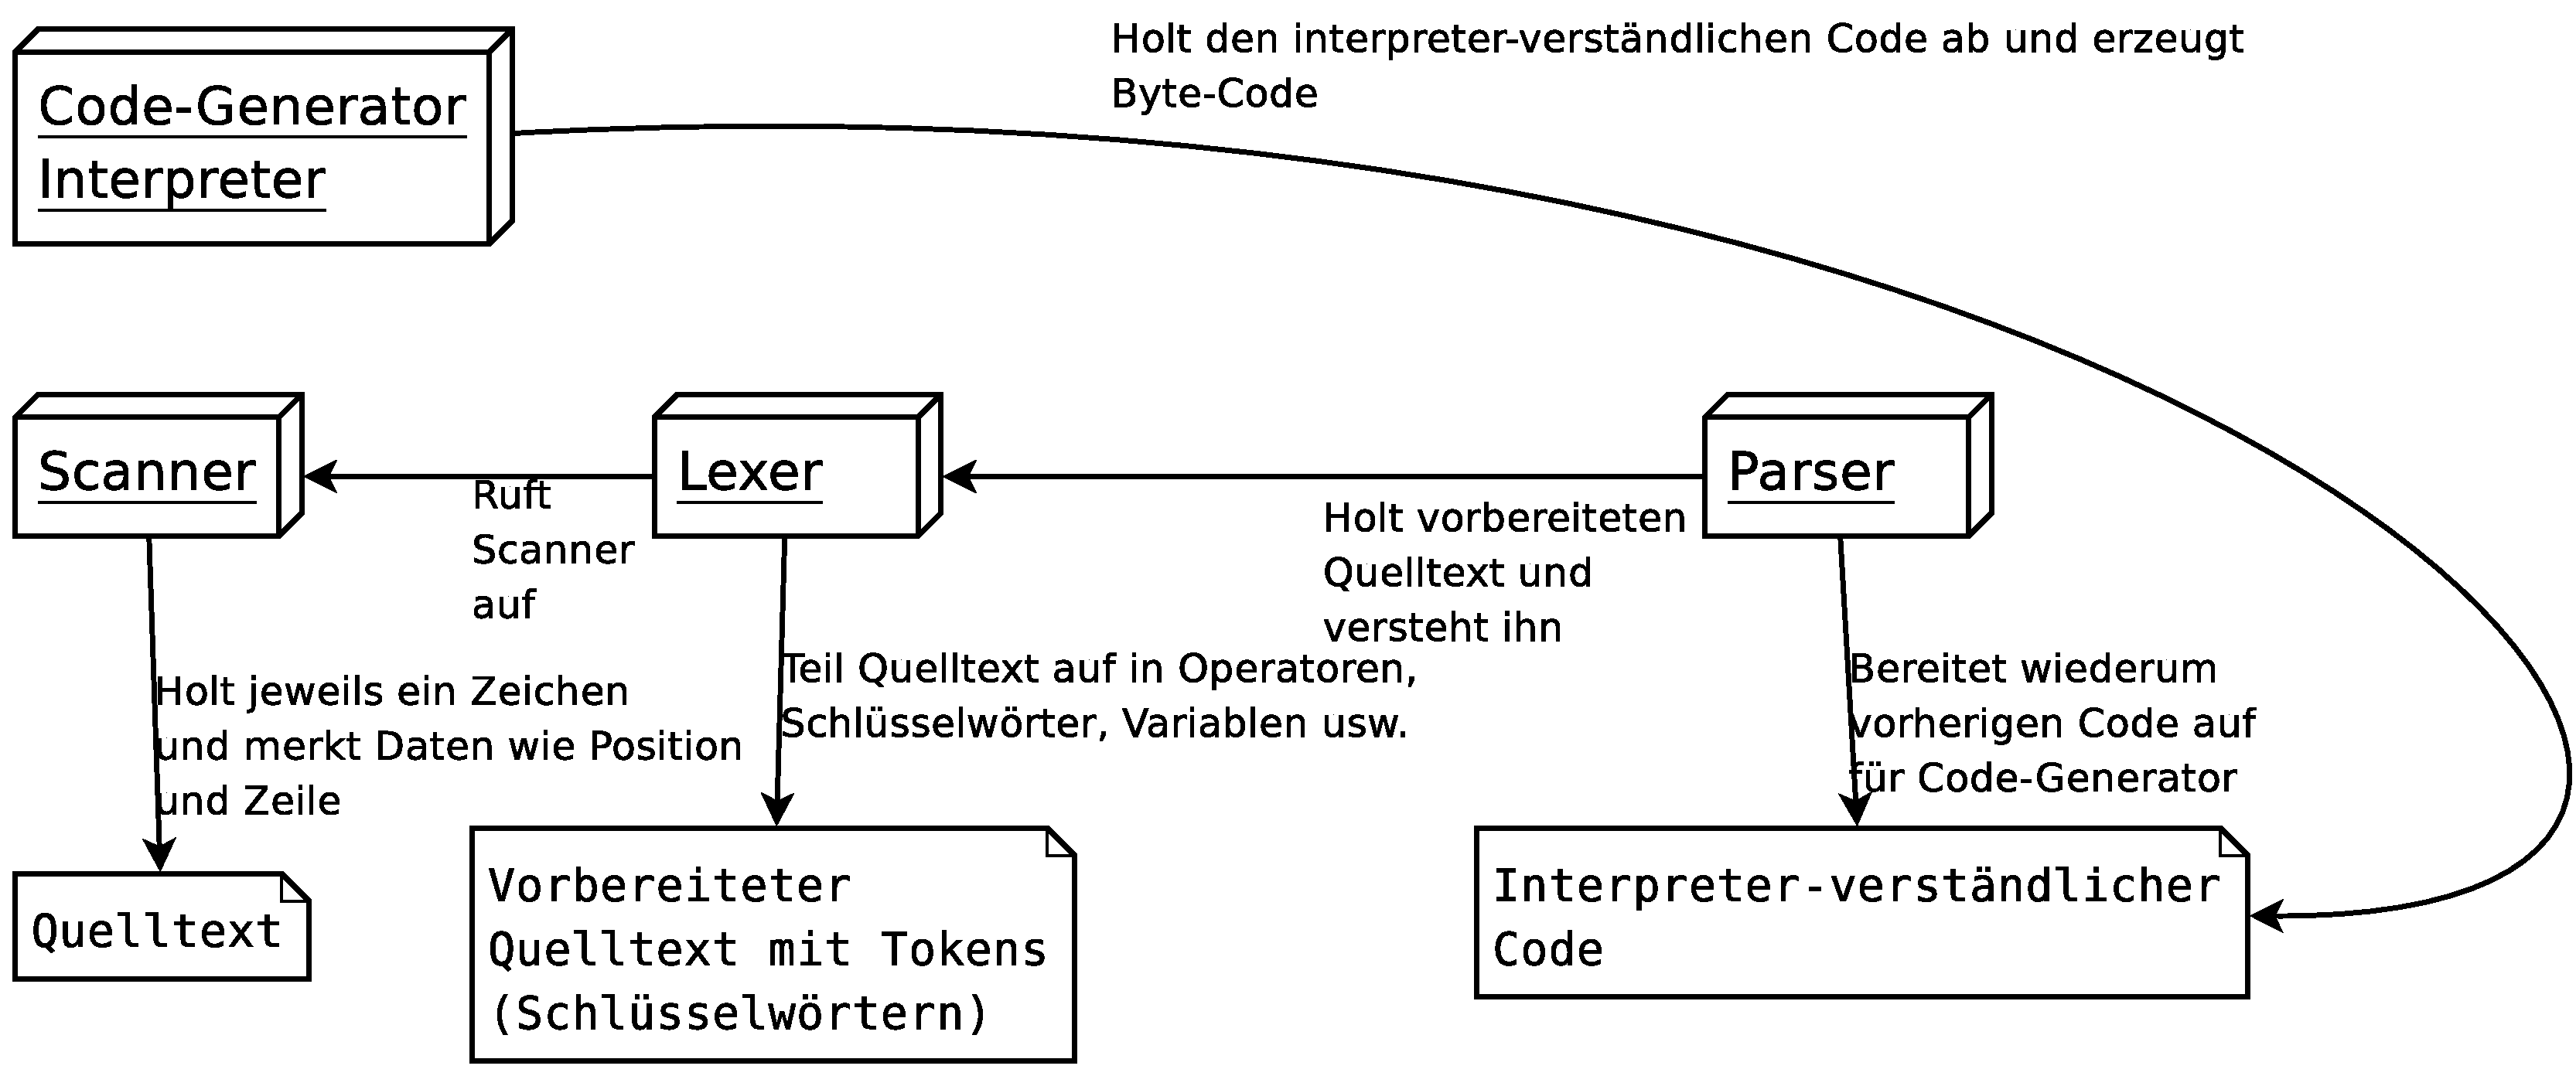
\includegraphics[width=15cm]{interpreter-diagramm.eps}
\newline
\subsection{Der Scanner}
Beginnen wir mit der am Häufigsten verwendeten und wichtigsten Einheit des Interpreters: Dem \emph{Scanner}.
Der Scanner hat eigentlich eine ganz simple AUfgabe. Er liest jedesmal, wenn der \textbf{Lexer} ihn aufruft, ein Zeichen aus dem Quelltext und übergibt es ihm. Dabei hat der Scanner einen internen Zähler, damit er weiss wo er gerade hinzeigt, einen sogenannten \textbf{Zeiger}. Dieser lässt sich nach vorne und nach hinten bewegen.
\subsection{Der Lexer}
Der \emph{Lexer}, oft auch \emph{Lexxer} genannt, ist ein sogenannter \textbf{Lexikalischer Scanner}. Er zerlegt die Textdaten, welche er vom Scanner erhält in logische Einheiten und ordnet sie in der korrekten Reihenfolge zu und verknüpft das Nötigste.\newline
Das Zerlegen in diese \textbf{Tokens} (Teilstücke eines Textes) geschieht dabei nach fest vorgebenen Regeln, also einer gewissen Grammatik, die von Anfang an definiert worden sein muss. Heutzutage wird dieser Teil bei der Entwicklung eines Compilers oder Interpreters nicht mehr selbstgeschrieben sondern man entwickelt freie Software dazu; so exisiteren zum Beispiel das in UNIX-Systemen enthaltene oder dafür frei verfügbare \emph{Lex} oder andere Programme für diese Aufgabe, die einem die Aufgabe des Zerlegen des Quelltextes in Token abnimmt. Die Regeln, sprich: Grammatik dafür, muss jedoch weiterhin selber geschrieben werden.
\subsection{Der Parser}
Der \textbf{Parser} baut nun auf das Vorwerk der Lexer und Scanner auf und sorgt nun dafür, dass logisch Fehler erkannt werden und strukturiert die vorbereiteten Daten. Ein Parser kann aber nicht nur in der Compiler-/Interpreterentwicklung nutzvoll sein. Auch bei der HTML-Programmierung wird z.B. ein Parser verwendet, um den Code zu analysieren und strukturieren, bzw. verständlich zu machen für den \emph{Internet-Browser}.
\subsection{Der Compiler/Interpreter}
Kommen wir letzten Endes zum \textbf{Compiler/Intepreter}; man könnte meinen, dies sei der wichtigste Teil, aber beim ganzen Prozess kommt keine Komponente ohne die andere aus.\newline
Der Interpreter erzeugt Im Falle von Python \textbf{Byte-Code}, eine Art Zwischenstufe zur endgültige, binären Maschinensprache, die beim ausführen eines Python-Interpreters leichter verstanden wird und zur höheren Geschwindigkeit bei der Ausführung der Programme dient. Ein Compiler hingegen würde hier nicht Byte-Code ausgeben sondern bereits \textbf{Objekt-Dateien} ausgeben. Objekt-Dateien enthalten Symbolen zu Funktionen und Variablen und enthalten letzten Endes eigentlich bereits \emph{Binärcode}. Der letzte Schritt fehlt hier aber noch, dieser ist nur für Linker relevant.
\subsection{Der Linker}
Ein \textbf{Linker} löst die verschiedenen Verknüpfungen von den Objektdateien zu Bibliotheksdateien, welche die Funktionen beinhalten auf und erzeugen am Schluss eine ausführbare Datei. Das endgültige Kompilat quasi, welches wir dann ausführen können. Bei Python ist dies nur über Umwege möglich, bei \emph{C/C++} ist dies aber der normale Weg, den werden wir später noch kennenlernen.
\newline
Ich hoffe damit ein Grundverständis erzeugt und nicht noch mehr Verwirrung gestiftet zu haben, aber das alles müssen Sie noch nicht verstehen. Aber es ist bestimmt hilfreich zu wissen, was genau hinter den Kulissen passiert, wenn wir ein Programm ausführen und kompilieren.
\part{ANSI-C-Kurs für Anfänger}
\label{part:ansic}
\chapter{Hintergrundwissen}
\section{Entwicklung und Geschichte von C}
C gehört zu den sogenannten Hochsprachen und wurde in den 1970'er Jahren entwickelt von \emph{Ken Thompson} und \emph{Dennis Ritchie} in den Bell Labs. Ursprünglich, als eine der ersten Hochsprachen, gab es \emph{ALGOL 60} die etwa 1960 entwickelt worden war von einem internationalen Komitee.

Daraus wurde dann \emph{CPL} (\textbf{C}ombined \textbf{P}rogramming \textbf{L}anguage) geschaffen, woraus dann wiederum \emph{BCPL} (für \textbf{B}asic \textbf{CPL}) entstand. 1970 entstand dann einer der direkten Vorgänger von dem, was später als (ANSI-)C zu weltweiter Verbreitung finden sollte: Simpel und schlicht \textbf{B} wurde es genannt.

Vielen ist bekannt, dass wir die Entwicklung der Programmiersprache \emph{C} den Bell Laboratories zu verdanken haben, welche im Zuge Ihrer Planung und Entwicklung von \emph{UNIX} das System später sogar in C schrieben.
Denn zunächst entstand durch die beiden Entwickler \emph{Ken Thompson} und \emph{Dennis Ritchie} am \emph{MIT} das \emph{Betriebssystem UNIX}, und zwar noch in \textbf{Assembler}\footnotetext{Maschinensprache: Für den Computer direkt verständliche Codes (\emph{Mnemonics}).}.
\newline

\section{C kommt - und bleibt!}
Da Assembler nicht gerade leicht gerade gut lesbar und verständlich ist aufgrund ihrer Struktur und der verwendeten Zahlensysteme, reifte in den beiden Entwicklern der Wunsch, eine einfache wie schnelle Programmiersprache zu entwickeln, welche nicht bloss auf einem Rechner lauffähig sein sollte, sondern auf jedem Rechner lauffähig sein sollte ohne grosse Anpassungen am Quelltext vornehmen zu müssen.\newline
Der grosse Nachteil in Assembler lag nämlich besonders darin, dass für nahezu jeden Prozessor wieder ein teilweise komplett anderer Befehlssatz offeriert wurde, hinzu kamen andere Eigenheiten wie verschiedene \textit{Byte-Reihenfolgen}\footnotetext{Lesen Sie dazu bitte das Kapitel $\rightarrow$\emph{Little Endian vs. Big Endian - Byte-Reihenfolgen und ihre Auswirkungen} und systemspezifische Arten der Speichernutzung.}

Da nun \emph{UNIX} eben aus oben genannten Gründen nicht auf allen Systemen lauffähig war, beschloss der junge Wissenschaftler \emph{Dennis Ritchie}, eine Sprache zu entwickeln, die für solche performantenwie portablen Applikationen, bzw. deren Entwicklung, geeignet war und schuf auf einer \emph{PDP-11}, ein damals weitverbreiteter Grossrechner, im Jahr 1971 auf Basis der Programmiersprachen \textbf{BCPL} und \textbf{B} endlich die erste Version von \emph{\textbf{C}}!

Schon bald darauf folgte die Feuertaufe im Jahre 1972 für \textbf{C}: \textbf{UNIX} wurde nun von \emph{\textbf{Assembler}} in \emph{\textbf{C}} umgeschrieben und für den \textbf{PDP-11} veröffentlicht.\newline
In den nächsten Jahrzehnten sollte es sich auf der ganzen Welt rasant verbreiten und weiterentwickeln. Ursprünglich nur für Grossrechner und die Industrie gedacht, verbreitete es sich in den 80'er Jahren ebenfalls dank der ersten Umsetzungen für Intel-Rechner auf Home-Computer von Privatleuten, welche dank \textbf{UNIX} die Kapazität ihrer Heimrechner immer mehr ausnutzen wollten und erstmals konnten. Eine der erfolgreichsten, \textit{unixoiden} (sprich: \emph{\textbf{UNIX}	}-ähnlichen) Betriebssysteme hat weltweite Verbreitung auf alle möglichen Arten von Prozessoren und Rechnern gefunden und ist uns heute bekannt unter dem Namen \textbf{Linux}!
\section{Grossvater UNIX und Stiefenkel Linux}
Ganz im Sinne der Entwickler haben sich \emph{\textbf{UNIX}}, bzw. heute vermehrt auch \emph{\textbf{Linux}} weltweit überwiegend auf Servern, aber auch auf Client-Rechnern, verbreitet und wurden auf alle möglichen Plattformen portiert. Nicht zuletzt verdankt man diesen grossen Erfolg  der \textbf{GPL}-Lizenzierung \footnote{Mehr Informationen und Hinweise hierzu finden Sie im Kapitel "'Programmieren unter Linux"`}, die einen grossen Teil zur Popularität und öffentlichen Beteiligung beigetragen hat durch Offenlegung der Quelltexte.

Und genau wie sein Urahn UNIX wurde Linux zu einem überwiegenden Teil in \emph{C} geschrieben.
Die meisten Distributionen\footnote{Distributionen sind Zusammenstellungen von Linux-Software mit Linux als Kern(el). Sie werden von kommerziellen Betreibern und der privaten Linux-Community erweitert, gepflegt und gewartet.} liefern heute standardmässig einen C-Compiler (üblicherweise den \emph{\textbf{gcc}} $\rightarrow$ \emph{\textbf{GNU C Compiler}}) und den Quelltext zur Distribution mit; so wird dem Benutzer gleich von Anfang an eine Entwicklungsumgebung zur Verfügung gestellt, die ihm erlaubt, das System nach seinen Wünschen anzupassen oder zu verändern, bzw. sogar Fehler zu berichtigen und Features zu programmieren, welche er in die Distribution zurückfliessen lässt und somit zur ständigen Weiterentwicklung beiträgt.

Um nocheinmal zu C zurückzukommen: Durch die Vervielfältigung des sich ständig in Wandlung befindlichen Betriebssystems UNIX / Linux, gab es während den 70'er und 80'er Jahren keine eindeutige Definition, welchen Sprachumfang C nun genau umfasst.

So besitzt C zum Beispiel kaum eigene Funktionen, liefert jedoch im Standardumfang div. Funktionen wie z.B. \textbf{printf()} zur flexiblen Textausgabe mit, welches wohl jedem von "'Hello World"`-Programmen bekannt ist.
Um einer weiteren wilden Verbreitung unkontrollierbarer und inkompatibler Derivate Einhalt zu gebieten, wurde vom \textbf{ANSI} (\emph{\textbf{A}merican \textbf{N}ational \textbf{S}tandard \textbf{I}nstitute}), einem Komitee zur Festlegung und Festigung von Standards in vielen verschiedenen Gegenständen und Technologien des alltäglichen Gebrauchs. Diese dienen zur besseren Interkommunikation und Zusammenarbeit zwischen Institutionen, Firmen und letztendlich Menschen und optimieren diese.

1988 gab es somit die erste Sprachbeschreibung des ANSI und ein Jahr später erreichte eben diese Sprachbeschreibung den offiziellen Status eines ANSI-Standards und wird seither als \textbf{\emph{ANSI-C}} bezeichnet \lbrack wie in diesem Buch natürlich auch.\rbrack
\newline
\section{Über ANSI-C und C++}
Wie schon früher angedeutet und hingewiesen, ist \textbf{ANSI-C} eine flexible, portable Programmiersprache, die auf fast allen gängigen aber auch selteneren Betriebssystemen zur Verfügung steht und untereinander weitestgehend kompatibel sind, da die Sprache den \emph{ANSI-Standard} von C hält und somit keine allzugrossen Differenzen bei der Funktionalität entstehen.
Mit dem Erlernen von C investieren Sie in ein zukunftssicheres Wissen, welches auch in 20 Jahren in den Prinzipien noch seine Gültigkeit haben wird; desweiteren wird man ihre heute in \emph{ANSI-C} entwickelten Programme ebenfalls noch viele Jahre lang lauffähig übersetzen können.

Durch die hohe Verbreitung von \emph{C und C++} ist dieses Wissen in kommerzieller als auch, sogar insbesondere, in non-kommerzieller (\emph{Open-Source, Hobby-Entwickler}) Hinsicht hochgefragt.

Was mit \textbf{Linux}, \textbf{UNIX} und \textbf{Mac OS X} (\emph{\textbf{Objective-C}}), eignen sich diese Sprachen perfekt zur Systemprogrammierung. Darüberhinaus werden die C-Sprachen auch noch eingesetzt für Treiberentwicklung und für die Anwendungsentwicklung auf eingebetteten Systemen/Mikrocontrollern.

Die meisten der heutigen kommerziellen Anwendungen werden in \emph{\textbf{C oder C++}} geschrieben. Vermehrt kommt seit einigen Jahren auch \emph{Java} zum Einsatz, da im Gegensatz zu \textbf{C/C++} die Quelltexte von \textbf{Java} nur ein einziges einmal kompiliert werden müssen und Anschluss auf jedem System, welches über eine \textbf{\textbf{JVM}}\footnote{Java Virtual Machine - Eine virtuelle System-Umgebung, in der Java-Anwendungen ablaufen} verfügt, in der Lage ist, die Programme laufen zu lassen.

Es ist heutzutage offensichtlich, dass immer mehr Wert darauf gelegt wird, dass Programme leicht auf mehreren Plattformen lauffähig sind, und, wie schon erwähnt, bieten \textbf{C} und \textbf{C++} genau diese Möglichkeit, den Quelltext ohne (grössere) Änderungen auf jeder Plattform zu übersetzen. Einer der weiteren Vorteile ist die geringe Speichernutzung, bzw. das optimale Speichermanagement, worin besonders C++ punkten kann. Nach C/C++ sind meistens nur noch Assembler-Anwendungen kleiner, welche jedoch nicht annähernd über dieselbe Flexibilität verfügen.

Um das Augenmerk auch noch ein wenig auf \emph{C++} zu lenken: C++ verfügt gegenüber C viele Vorteile. C++ selber ist eine \emph{Obermenge} von C, das heisst: Alle Elemente von C sind in C++ auch enthalten; darüberhinaus besitzt C++ jedoch noch viele weitere Fähigkeiten, die in der modernen Software-Entwicklung nicht mehr wegzudenken wären.

Dazu gehören unter Anderem:\newline

\begin{itemize}
 \item Objektorientierung: Bietet eine bessere Ordnung und Verwaltung von Projekten.
\item Die Speicherverwaltung ist mit \emph{new} und \emph{delete} weitaus absturzsicherer, einfacher und sauberer geworden. Vorallem ist die Allokation von Speicher nun Hauptbestandteil von C++ selber.
\item Die Objektorientierung bringt \emph{Vererbung} mit sich; das bedeutet, dass Klassen nun (in C bekannt als Funktionen:)Methoden und (Variablen:)Attribute von anderen Klassen erben können, während man in C noch komplett neue Strukturen und Funktionen schreiben musste.
\item Das Stream-Konzept: Daten werden in Form von Datenströmen, Streams, gelesen und geschrieben
\item Konstruktoren und Destruktoren: Beim Erzeugen und Löschen einer Instanz einer Klasse, werden selbstdefinierte Funktionen, den Konstruktor und den Destruktor, ausgeführt. Ideal um z.B. dazugehörigen Speicher gleich mitzulöschen, damit er nicht im Speicher hängenbleibt.
\item Polymosphirmus: Darauf gehe ich in C++-Kurs näher ein, da das hier sonst den Rahmen sprengt.
\end{itemize}
\subsection{C-Standards und dieses Buch}
Ich habe in diesem Buch bewusst den ANSI-C-Standard \textbf{C99} durchgehend benutzt; dabei muss man weiterhin unterscheiden zwischen verschiedenen Revisionen des Standards. So gab es neben dem ursprünglichen (nicht-ANSI-)\textbf{K\&R-C} (logischerweise \emph{Kernighan \& Ritchie-C}) von \textbf{1978} die ANSI-Varianten \textbf{C89, C90} und \textbf{C99l}; die Zahl steht dabei stellvertretend für die Jahreszahl der Veröffentlichung\newline Dabei profitierten die späteren Revisionen von den Neuerungen seines weiterentwickelten Bruders \textbf{C++}, von dem viele Funktionen und Definitionen zurückflossen nach \textbf{C}.

Einige kleine Beispiele von \textbf{C99} im Vergleich \textbf{K\&R-C}:

\begin{itemize}
 \item Der zeilenweise Kommentar wurde ergänzend zum altbekannten "\textbf{/* ... */}" von \textbf{C++} übernommen.
\item Die Variable \textbf{void} wurdei ns Repertoire der Sprache aufgenommen.
\end{itemize}


\chapter{Voraussetzungen und Software}
Um für Ihr gewünschtes System programmieren zu können, benötigen wir neben einem ganz normalen Text-Editor, wie er bei jedem heutigen Betriebssystem dabei sein sollte, einen Compiler. Der Compiler übersetzt unseren Quelltext in eine für das Zielsystem verständliche Sprache; in unserem Fall wird das Ergebnis \emph{Maschinensprache}. Bei Java wäre es hingegen \emph{Bytecode}, eine Art Maschinensprache für die \textbf{Java Virtual Machine}(JVM), welche einen virtuellen Computer darstellt. Diese Virtual Machines gibt es für jedes gängige Betriebssystem und daher verstehen diese Systeme dank der \emph{JVM} diesen Bytecode. Das ist das \textsc{Geheimnis} hinter der Portabilität von Java und läuft daher überall. \newline

Bei C müssen wir uns hingegen damit begnügen, dass die Programme jeweils nur auf der gewählten Plattform (Prozessor und Betriebssystem)  läuft, für die kompiliert wurde. Deswegen müssen wir auch für jedes System ein neues Kompilat erzeugen. Jedoch können wir, insofern wir nicht zuviele systemspezifische Anpassungen vorgenommen und uns weitestgehend an den ANSI-C Standard gehalten haben, dazu immer denselben Quelltext verwenden ohne Änderungen daran vornehmen zu müssen, was zu einer stark erhöhten Portabilität führt.
\\\newline
\section{Die Basis - Das Betriebssystem}
Wie wir nun bereits aus dem vorherigen Linux-Kapitel wissen, ist Linux nicht gleich Linux: Es gibt auf dem Markt zahlreiche mehr und weniger erfolgreiche Distributionen. Zu den erfolgreichsten Distributionen mit einer grossen Benutzer- und Entwicklergemeinde zählen \textbf{Ubuntu, Debian, OpenSuSE, Mandriva, Red Hat} und {textbf}. Daneben gibt es, wie bereits erwähnt, zahlreiche weitere Distributionen, die auf spezielle Intentionen und Anwendungszwecke ausgelegt sind und eher für kleinere Nischenbereiche eingesetzt werden.\\
Selber verwende ich Ubuntu Linux, welches ein Ableger von Debian Linux ist und somit dasselbe Paketsystem benutzt (\textbf{APT}), jedoch gegenüber Debian um ein Vielfaches für Neueinsteiger in die Linux-/Unix-Welt vereinfacht wurde durch graphische Oberflächen und Tools, die der einfachen Konfiguration des Systems dienen.\\
Wahrscheinlich verwenden Sie bereits eines dieser Systeme und können bereits damit umgehen; falls Sie jedoch noch absolut nicht vertraut im Umgang damit sind, rate ich Ihnen zu \emph{Ubuntu Linux}. Schliesslich wollen wir uns nicht mit Konfigurationsproblemen aufhalten, sondern so schnell wie möglich zum Programmieren übergehen, oder?
\\
\section{Compiler - Unterschiedliche Standards und Versionen}
Ob und wie der Quelltext kompiliert wird, hängt natürlich dann wiederum jeweils davon ab, welchen Compiler wir verwenden, denn die verschiedenen Hersteller halten sich nicht immer an die Standards und führen diverse Eigenheiten ein, die zwar von Vorteil sein mögen für einen Programmierer, sich jedoch zum Hindernis entwickelt, wenn dieser Compiler nicht für jeden verfügbar ist, der das Programm für seine Zwecke kompilieren möchte.\\\newline

Aus diesem und anderen Gründen habe ich mich dazu entschlossen, ausschliesslich \emph{freie Software} zu verwenden für die Programme in diesem Buch. Zusätzlich zu dem Nebeneffekt, dass ich damit ein wesentlich grösseres  Zielpublikum erreiche, kann sich jeder interessierte Leser mit Internet-Anschluss gratis die benötigte Software herunterladen und alle Programme im Buch selber kompilieren o. verändern um sie nachvollziehen zu können oder natürlich selber welche zu entwickeln. Denn in erster Linie soll dieses Buch ja anregen zur Eigeninitiative des Lesers und zur Umsetzung von eigenen Ideen, nicht dem Bau von Software-Plagiaten.
\\
Als Compiler verwende ich folglich den \textbf{GNU C Compiler} (\emph{GCC}), welcher sich weitestgehend an ISO-Standards hält. Er bietet den Vorteil, dass er für nahezu jede Platform, auf der Linux oder Unix zu finden ist, ebenfalls zur Verfügung steht, selbst für Windows ist mittlerweile eine Version veröffentlicht worden. Somit sollte keiner darin behindert sein, aktiv bei diesem Buch mitzumachen bei den Übungen und Beispielen. GCC sollte bei Ihrer Linux-Distribution über den Paketmanager erhältlich sein wenn Sie nach 'gcc' suchen.
\\\newline
Auf jeden Fall können Sie beruhigt sein, denn auch wenn Sie eine andere Programmierumgebung besitzen oder verwenden möchten, sind Sie auf der sicheren Seite. Da sich die Programme in diesem Buch an den ANSI-C Standard halten, sollten sie auf allen gängien Compilern auch kompilierbar sein. Getestet habe ich die Programme jedoch alle selber nur unter \emph{einer Linux Umgebung mit GCC in der Version 4.1.2}.
\section{Editoren - Die Qual der Wahl}
Als Editor dient, wie schon erwähnt, das, was für Sie am Besten passt In der Vielzahl der unzähligen Editoren gibt es spezielle Editoren, die u.A. \emph{Syntax Highlighting} besitzen. Das bedeutet, dass Sie den Quelltext farbig markieren bei Schlüsselwörtern und den entsprechenden Zeichen. Dies erleichtert dem Betrachter enorm das Verständnis des Quelltexts. Desweiteren gibt es noch die Funktion, Compiler auszuwählen und per Knopfdruck ganze Kompilierprozesse automatisiert ablaufen zu lassen oder letzten Endes sogar das Programm selber.

Solche Programme werden auch \textbf{Integrated Development Environment}(\emph{IDE}), eine \textsc{integrierte Entwicklungsumgebung}, genannt und sind eine elegante Art und Weise, um organisiert und bequem Projekte/Programme zu entwickeln, die einen etwas grösseren Umfang besitzen. Gleichzeitig eignen sie sich natürlich für Anfänger dank der vielen Hilfsfunktionen.
\\\newline
In diesen Umgebungen lässt sich bequem arbeiten dank vieler Erweiterungen wie Syntax-Fehlererkennung, Textsuche, Umrechner usw.
Zu den beliebtesten Programmen gehören dabei die beiden Java-Anwendungen \textbf{NetBeans} (http://www.netbeans.org) und \textbf{Eclipse} (http://www.eclipse.org). Beide sind frei erhältlich und stehen unter Lizenzen, die den Quelltext ebenfalls zur Verfügung stellen. Sie lassen sich jedoch nicht nur für C oder C++ einsetzen, sondern für eine Vielzahl anderer Programmiersprachen. Die Bandbreite reicht dabei von Java bis zu PHP, je nachdem welche Erweiterungen man geladen und welche Compiler man installiert hat. Zumal Sie eigentlich anfänglich auf Java ausgerichtet waren und auch dafür geschaffen worden sind ohne die meisten Plugins.
Persönlich bevorzuge ich den etwas aktuelleren NetBeans, der über eine Vielzahl an Plugins verfügt. Man denke alleine an die Versionierung und das Backup Ihrer Quelltexte...!
\chapter{Datentypen}
Wenn wir programmieren, müssen wir temporär Daten in Form von Bytes im Speicher lagern. Diese bekommen einen Platz, \textbf{Variable}, zur Aufnahme zugewiesen. Dabei müssen wir beachten, \emph{wie} wir sie ablagern möchten und wie der Computer sie zu verstehen hat. Deswegen müssen die Variablen in bestimmten Datentypen deklariert werden. Zudem brauchen auch Funktionen\footnote{Sequenzen von Programmcode irgendwo im Speicher, die man immer wieder aufrufen kann.} einen Datentyp, denn eine Funktion gibt nachdem sie aufgerufen wurde einen Wert zurück, nämlich das erwartete Resultat der Funktion.

Wenn wir zum Beispiel eine Funktion haben, die uns eine Zahl multplizieren soll, dann wissen wir, dass wir eine Ganzzahl (Integer) zurückbekommen möchten, wenn wir normale Dezimalzahlen verwenden. Wichtig zu wissen ist für uns auch, wieviele Bytes eine Variable zugewiesen bekommt im Speicher, damit wir wissen, wieviel Speicher/Variablen wir eines Typs benötigen um z.B. eine Datei komplett in den Speicher laden zu können.

\emph{C} verfügt über eine ganze Reihe von Datentypen, die in verschiedener Konstellation mit zusätzlichen Attributen deklariert werden können.
In den folgenden Unterkapiteln gehe ich auf jeden enizelnen Datentyp und seine Verwendung genauer ein anhand eines analytischen Beispiels.
Um Ihnen zuvor einen besseren, groben Überblick zu verschaffen, habe ich die Datentypen in einer Tabelle zusammengefasst:
\begin{center}
\begin{table}[h]
\caption{Eine Tabelle mit C-Datentypen und ihrer Anwendung.}
\begin{tabular}{|l|c|c|c|r|}\hline
Datentyp & Schlüsselwort & Bytes & Verwendung & Zahlenraum\\\hline\hline
Buchstabe(Character) mit Vorzeichen & signed char & 1 & Buchstaben und Sätze & -128..127\\\hline
Buchstabe(Character) ohne Vorzeichen & unsigned char & 1 & 0..255\\\hline
Ganzzahl(Integer) mit Vorzeichen & long int & 8 &\\\hline
Ganzzahl(Integer) mit Vorzeichen & int & 4&\\\hline
Ganzzahl(Integer) ohne Vorzeichen & short int & 4&\\\hline
Fliesspunktzahl(Floating Point) nur mit Vorzeichen & float & 4&\\\hline
Fliesspunktzahl(Floating Point) nur mit Vorzeichen & double & 8&\\\hline

\end{tabular}
\end{table}
\end{center}
\chapter{Einführung in die Sprache C}
Das kleinstmögliche Programm in der Sprache \emph{C} sieht folgendermassen aus:
\begin{verbatim}
 main()
{
}
\end{verbatim}
Es führt eigentlich nicht wirklich etwas aus und beendet sich sofort wieder, doch sehen wir hier schon einmal die elementaren Bestandteile jedes C-Programms.
Ein C-Programm besteht immer aus Funktionen. Funktionen sind Code-Sequenzen, die man beliebig aufrufen kann, sofern sie deklariert und definiert sind. Ein Programm, das zum Beispiel dafür geschrieben wurde zum Berechnen von Zahlen, wird mehrere Funktionen aufweisen wie zum Beispiel Addieren(), Subtrahieren() oder Ähnliches. Die Hauptfunktion heisst dabei immer gleich, nämlich wie im obigen Beispiel \textbf{main()}.\\
Eine Funktion gibt normalerweise immer einen Wert zurück, zum Beispiel das Ergebnis einer Addition oder ob die Addition erfolgreich verlaufen ist oder nicht. Die Art des Wertes muss natürlich auch definiert werden, Funktionen haben also immer einen bestimmten Datentyp. Den Datentyp stellt man vor die Funktion bei der Deklaration, jedoch nicht beim Aufruf.

\chapter{Das erste Programm}
Für Ihr erstes C-Programm, können Sie untenstehenden Quelltext verwenden; diese Anwendung liest über die \textbf{Standardeingabe (STDIN)}, in Ihrem Fall die Tastatur, einen String ein. Jener String darf maximal 15 Zeichen betragen, da nicht mehr Speicher alloziiert worden ist, und wird nach der Eingabe mit Return in das Programm übergeben, welches diesen Satz anschliessend auf der \textbf{Standardausgabe (STDOUT)}, dem Bildschirm, ausgegeben.
\newpage

\part{Der C++-Kurs}
\label{part:cpp}
\chapter{Hintergrundwissen}
\section{Entwicklung und Geschichte von C++}
\emph{C++} wird vielen Anwendern wie Programmierer heute ein Begriff sein, galt und gilt sie doch seit Jahren als meistverwendete Programmiersprache im kommerziellen Sektor. Als objektorientierte Hochsprache hat C++ den Trend gesetzt und seit seiner Veröffentlichung in den 1980'er Jahren einen enormen Popularitätsschub sowie viele Nachahmer, teils zweifelhafter Qualität, bekommen. Meist gilt C++ immer noch als zentrales Herzstück der IT-Industrie, aber mittlerweile haben nicht weniger vielversprechende Hochsprachen C++ eingeholt und sind auf zeitgemässe Wünsche von Anwendern und Entwicklern eingegangen. \emph{Java}, \emph{C\#} oder gar \emph{D} sind nur eine kleine Selektion der Sprachen, die mit C++ konkurrieren. Nichtsdestotrotz hat C++ immer noch einen Podestplatz in der Industrie inne und wird sich auch in den nächsten Jahren nicht davon runterstossen lassen, denn Tausende von Anwendungen basieren heutzutage auf dieser Sprache und werden es auch weiterhin, denn die performanten Anwendungen sind auch in Zeiten von zig-Gigabyte-Prozessoren nicht weniger wichtig und C++ ist äusserst flexibel!\\
So lassen sich heutzutage dank einer schier grenzenlosen Auswahl an Bibliotheken nahezu mit Leichtigkeit Programme aller Sparten entwickeln.\\
Während Programme anderer Sprachen plattformunabhängig sind, sind C++-Binäranwendungen plattformgebunden, gleich wie bei C lassen sich die Programme nur auf dem Prozessor ausführen, für welchen das Programm geschrieben wurde. In der Tradition von C hat aber auch C++ seine Portabilität bewahrt und lässt sich problemlos auf andere Plattformen portieren, desweiteren sind ale C-Programme in C++ kompilierbar, da C++ uneingeschränkt kompatibel zu ANSI-C ist.
\newpage
\part{Grundlagen der Netzwerktheorie}
\label{part:network}
\chapter{Einleitung}
\section{Netzwerke}
Netzwerke - jedes Unternehmen, jede Verwaltung und Millionen von Heimanwendern haben Computernetzwerke - das Bekannteste und Grösste von ihnen ist das \emph{Internet}. Sie sind in aller Munde und jeder, der was auf sich hält, hat Zugang dazu oder mindestens ein virtuelles Abbild seiner Selbst im digitalen Raum oder eine eigene Home Page. So sagt man zumindest; denn das Internet wie wir es heute kennen hat an sich nicht mehr viel zu tun, mit dem, wozu es ursprünglich geplant und konzipiert wurde.\newline
Dieser Part handelt das Thema Netzwerke mit einem Überblick über seine Facetten und Möglichkeiten ab; verzeihen Sie mir, dass ich nicht vollumfänglich in diese Thematik einsteigen kann, denn das würde schlichtweg den Rahmen eines Parts sprengen und ein ganzes Buch verlangen.
Den Schwerpunkt habe ich neben privaten und kommerziellen Netzwerken auf das Internet gelegt, welches ja im Grunde nichts anderes ist, als ein weltumspannendes Gebilde aus Computern/Servern/Anwendern. 
Am Anfang des Parts gehe ich auf allgemein bekannte Protokolle und Netzwerk-Strukturen ein, um einen groben Überblick zu verschaffen. Im Anschluss definiere ich das \emph{OSI-Modell} mit all seinen Schichten. So kann es also vorkommen, dass ich einige Schichten vorwegnehme und später möglicherweise nochmal (detailierter) behandle. Aus Gründen der einfacheren Verständlichkeit bitte ich Sie, dies zu beachten.
Was ich jedoch nicht bieten kann und werde sind detailierte \emph{PHP}-Progamme oder Erklärungen zu PHP selber, da dieses Buch definitiv andere Schwerpunkte im Mittelpunkt fixiert.

\section{Das Internet}
Charakteristisch für das Internet ist vorallem, dass jeder in der Lage ist, wenn er eine Server-Applikation oder Speicher auf einem Server im Internet besitzt, Daten im Internet zu hinterlegen für Andere. Dabei ist es völlig egal, was für Daten das sind, solange sie in einer vernünftigen Grösse vorliegen und sie gut zu erhalten sind. \newline
Übrigens, vielleicht werden Sie sich wundern, dass ich für das Internet manchmal diverse andere, durchaus gängige Begriffe verwende, wie zum Beispiel \emph{Web}. Abgesehen davon, dass es eine Vielzahl an Namen für das Internet gibt, verwende ich gerne Web, da das Internet auch bekannt ist als \emph{World Wide Web}, ein weit verstricktes, weltweites Netz also, ähnlich dem typischen Spinnennetz.
\chapter{Hintergründe zu Internet- und Netzwerktechnologien}
\section{Die Geschichte des Internets}
Liegen nun die Daten im \emph{HTML}-Format vor, dann können \emph{Browser}\footnotetext{Beispielsweise \emph{Firefox} oder der \emph{Internet Explorer} sind sogenannte Web-Browser, Navigationsprogramme im Internet.} diese Seiten interpretieren und formatieren, d.h. mit Farben und Text in verschiedenen Grössen und/oder mit Bildern verziert, darstellen. Besonders interessant ist die Fähigkeit, Texte und Bilder mit \emph{Links}, also Verweisen, zu versehen und den Benutzer so durch seine Website zu lotsen. Anhand einfacher Menüs und Auswahl-Hilfen wurde so eine optimale Übersicht über die Inhalte der Seite geboten und viele Websites verlinkten sich untereinander, um mehr Besucher anzulocken und andererseits um natürlich auch das Wissen zu verbreiten.\newline 
Das reizte zahlreiche (vorwiegend junge Fach-)Leute durch die vielfältigen Möglichkeiten des Internets dazu, sich der Web-Programmierung zu widmen und ihre Kenntnisse zu vertiefen. Dies führte dazu, dass nahezu alle \emph{Websites} in den Anfängen des Internet-Zeitalters zunächst in der einfach zu erlernenden ``Programmiersprache'' \emph{HTML} geschrieben wurden und bis heute hat sich daran eigentlich nichts geändert, ausser dass es mittlerweile mehr und mehr Funktionen und Möglichkeiten mit \emph{HTML} gibt. Ich schreibe es in Anführungszeichen, weil es keine eigentliche Programmiersprache ist, sondern eine Beschreibungssprache. \textit{HTML} fehlen die grundlegenden Eigenschaften von Programmiersprachen/Applikationen wie \emph{Schleifen}, \emph{If-Else-Bedingungen} und  \emph{Kompilierbarkeit in eine ausführbare Maschinensprache} (neben vielen Anderen...!). Diese Einschränkung lässt sich jedoch mit Hilfe von Erweiterungen/Zusatzprogrammen für den \emph{Webserver} (die Applikation, die den Dienst auf dem Rechner im Internet anbietet, oftmals sind es der \emph{Apache}-Webserver oder der \emph{IIS}) umgehen.
\chapter{Netzwerk-Typen}
Es gibt verschiedene Arten, wie man ein Netzwerk strukturell aufbauen kann. Dabei beziehen sich die Differenz hauptsächlich auf die Hierarchie und die Verkabelung des Netzwerks. Es ist also wichtig von Anfang an zu wissen, zu welchem Zweck ein Netzwerk aufgebaut wird und für welchen Zeitraum, denn so fällt die Wahl für das jeweilige System sehr einfach. Grundsätzlich empfiehlt sich jedoch das \emph{Client-Server-Prinzip} als langfristige Lösung, wenn eine stabile und sichere \emph{Backup-Lösung} vorhanden ist.
\section{Das Client-Server-Prinzip}
Wenn wir beispielsweise nun eine Adresse eingeben würden, auf der ein Webserver läuft, würde der Browser auf dieser Adresse nach der Datei \emph{index.html} oder \emph{index.php} anfragen und der Dienst nach dieser Datei auf seinem Rechner suchen. Je nach Einstellung, sucht er, wenn keine spezielle Seite angegeben wurde sondern nur der Domänenname (beispielsweise \url{http://www.google.com}), nach einer Startseite, die dann wiederum weiterlinkt zu anderen Seiten.
Hier haben wir also das sogenannte \emph{Client-Server-Prinzip}. Verdeutlichen wir die Situation am Besten anhand einer Allegorie: Wir nehmen also an, dass der Client quasi ein Kunde in einem riesigen Warenhaus (= Netzwerk/Internet) darstellt und der Server der Verkäufer oder Auskunftgeber. Der Verkäufer bietet in seinem Laden vielleicht nun einen Service an, an dem wir interessiert sind und vondem wir  vielleicht bereits irgendwo auf einem Plakat oder in einem anderen Laden ( = einer anderen Website) gelesen haben. Also fragen wir ihn nach dem Sonderangebot, dass die Marketing-Abteilung des Unternehmens, zu dem das Geschäft gehört, inseriert hat. Nachdem sich der Verkäufer in seinem aktuellen Katalog sich erkundigt hat, sagt er uns wo wir den Artikel finden, beziehungsweise ob er überhaupt noch vorhanden ist, sonst gibt er eine `Fehlermeldung` aus. Ist der Artikel nun vorhanden im Laden und gibt er ihn uns und studieren ihn.\newline

Wir haben uns jetzt die 2 verschiedenen Grundrollen angeschaut. Es gibt einen Dienstleister und einen Empfänger der Dienstleistung. Der Kunde benötigt im obigen Beispiel den Laden, weil er selber gar nicht in der Lage wäre, diesen Dienst an sich selbr auszuführen, also z.B. selber ein Kleidungsstück herstellen oder Nahrung zu fabrizieren, deswegen nutzen wir die Fähigkeiten eines Anderen, respektive sein Angebot. Wie im richtigen Leben sind nunmal auch im Internet nicht alle Dienste gratis, so kostet ja zum Beispiel alleine der Internetzugang schon etwas. Neben den üblichen Gratisdiensten wie \emph{Suchmaschinen, Übersetzer, Foren} und ähnlichen Services gibt es auch noch zahlreiche Anbieter, die von der Zahnbürste bis zum Kaviar alles online anbieten und man bequem von Zuhause oder vom Büro aus ordern kann. Es ist also nichteinmal mehr notwendig vor die Tür zu treten, um in den Genuss von frischen Nahrungsmitteln zu kommen. Oder vielleicht möchten Sie zur Abwechslung einmal eine Pizza vom Italiener...? Alles kein Problem.\newline
Wichtig zu erwähnen ist bei dieser Struktur, dass ein ausgeklügeltes \emph{Backup-Konzept} extrem wichtig ist, da hier alle Daten zentral auf EINEM Server (jedenfalls bei dieser Lösung, es gibt natürlich Schutzmassnamen und Notfall-Server in grossen Betrieben... aber eben nicht immer) gespeichert werden und somit ein grosses Sicherheitsrisiko darstellen. Somit sind Sicherheitskopien sehr zu empfehlen.\newline

Um zurück zum Client-Server-Prinzip zu kommen: Auf diesem Prinzip basiert die ganze Internet-Struktur und viele Netzwerke. Wir werden diese Struktur noch öfters antreffen bei anderen Protokollen, die genau gleich verfahren.

\section{Peer to Peer (P2P)-Netzwerke}
Auf vielfache Anfrage habe ich mich entschlossen, dieses Thema hier auch zu behandeln.
Dieser Abschnitt dient als kleine Exkursion und um eine Alternative zum vorher gezeigten \emph{Client-Server-Prinzip} aufzuzeigen. Hierbei gibt es nun einige Unterschiede:
Beim Client-Server-Prinzip sind die Teilnehmer beim Transfervorgang nicht gleichberechtigt, das heisst für uns, dass aus der Client-Sicht der Server mehr Macht hat, da er den ganzen Verbindungsvorgang abbrechen kann und schliesslich der Client etwas vom Server will und nicht umgekehrt.\newline
Das \emph{Peer to Peer-Prinzip} lebt hier praktischen Kommunismus vor: Alle `Peers`\footnotetext{Peer ist englisch und steht für `Gleichgestellter` oder `Ebenbürtiger`} sind sich in ihren Rechten und Fähigkeiten gleich. Und da speziell \emph{P2P} genutzt wird, um Daten unter vielen Benutzern untereinander auszutauschen, spielen alle Peers gleichzeitig Client und Server, da sie auch etwas anbieten müssen um das Objekt der Begierde erhalten zu können.\newline
Speziell hinzuweisen ist bei diesem System darauf, dass es gegenüber dem Client-Server-Prinzip einen entscheidenden Vorteil besitzt: Nahezu alle Daten sind \emph{redundant}, das heisst, sie sind doppelt vorhanden, auf mehreren Rechnern gleichzeitig dieselben Daten. Dies verbraucht zwar mehr Platz im Endeffekt, doch man braucht nicht um seine Daten zu bangen, die man beziehen möchte aus einem \emph{P2P}-Netzwerk. Besonders dann, wenn plötzlich einmal ein Rechner ausfällt, von dem man Daten bezogen hat, denn es findet sich meistens jemand anderes, der dieselbe Datei bereits vollständig besitzt und sie verteilt. Der klare Nachteil hingegen ist dafür dann eben, dass die Daten nicht zentralisiert erfasst sind und bestimmt kein normales Firmennetzwerk je nach so einem Schema aufgebaut wird. Wenn man an einer Gross-Veranstaltung (z.B. eine \textit{LAN-Party}\footnotetext{An LAN-Parties spielt man (meistens 3D-Shooter wie Quake oder Half-Life) Spiele im \emph{LAN} (Local Area Network, ein kleines Netzwerk) gegeneinander.) Daten verteilen will, ist so ein Netzwerk jedoch die beste Lösung, wenn man über keinen ständigen Server verfügt. }
\newpage

\chapter{Das HTTP-Protokol und die dynamischen Programmiersprachen}

Der Web-Dienst wirft die Daten im \emph{HTTP}-Protokoll aus zum Zielrechner, der die ursprüngliche Anfrage gestellt hatte. Das \emph{HTTP-Protokoll} steht für \emph{H}yper\emph{t}ext \emph{T}ransport \emph{P}rotocol und überträgt, wie der Name schon sagt, \emph{Hypertext}, aber auch andere Daten, über Netzwerke. Hypertext nennt man Texte/Dateien die sich untereinander verlinken können Mithilfe von Stichworten oder Bildern, die Verweise auf weiterführende Seiten/Dateien enthalten. Dies war eine neue, revolutionäre Funktion, denn man musste nicht mehr wie früher seitenweise durchscrollen/-blättern bis man zum gewünschten Programm oder zu einer dringenden Information gelangt, sondern konnte nun direkt von Punkt A nach Punkt B springen. Da die Seiten jedoch statisch waren und jede Menge Aufwand in der Wartung bedurften, kam bald der Wunsch auf, Websites doch dynamisch gestalten zu können. Die ersten Schritte in diese Richtung kamen dann mit den kleineren Skriptsprachen, welche zwar immer noch nicht wirklich dynamisch waren, aber bereits bewegte Bilder und Interaktivität bei kleinen Anwendungen und Spielen boten.
\section{Dynamische Programmiersprachen erobern das Web}
Weit verbreitet ist \emph{Javascript}, eine kleine Abwandlung von \emph{Java}, das aber eigentlich nicht allzuviel mit Java selber mehr zu tun hat, da ihm existenzielle Eigenschaften, die zu einer richtigen Programmiersprache wie \emph{Java} gehören, fehlen. 
So lassen sich z.B. keine Klassen definieren oder vererben. Es lässt sich jedoch auf Klassen-Objekte zugreifen und so lassen sich viele spezielle Funktionen in HTML-Seiten einbauen. Javascript wird oft für Effekte oder simple (\emph{unsichere!}) Passwort-Abfragen auf einer Seite verwendet, z.B. schwebende Schriften, (oft an Weihnachten) Schnee-Bilder die über den Bildschirm fliegen u.v.m.\newline Um jedoch zu den richtigen Programmiersprachen zu kommen: Es gibt hauptsächlich \emph{PHP} und \emph{ASP} und eigtl. noch diverse Andere, die aber mangels Verbreitung eher geringe Beliebtheit besitzen und bisher eher ein Nischendasein führten und es wohl auch weiterhin tun werden. PHP ist frei erhältlich / runterladbar von \url{http://www.php.net} und ASP benötigt eine Lizenz von Microsoft und lässt sich im Fachhandel oder über Microsoft(-Partner) beziehen. Aufgrund der riesigen Anhängerschaft, der guten Dokumentation \& Verfügbarkeit an freien Online-Kursen, empfiehlt sich \emph{PHP} als beste Wahl, falls man selber Web-Anwendungen entwickeln möchte. Die Sprachen dienen dem Zweck, dynamische Websites zu ermöglichen, während hingegen mit HTML alleine nur statische Websites möglich sind. \newline

Neu war bei diesen dynamischen Programmiersprachen, dass statt wie bisher bei \emph{Javascript} oder \emph{HTML} die Daten nicht mehr ausschliesslich lokal beim Zielrechner verarbeitet wurde, sondern nun jetzt, bevor der Server sie abschickt, individuell nach den Anforderungen des Anfrage-Stellers/Benutzers in HTML zusammenstellt und erst dann losschickt. Das heisst, dass letzten Endes dem Zielrechner auch wieder nur HTML-Date(ie)n über HTTP geschickt werden und keine Programmiersprache selber, sondern nur das Resultat ihrer Ausführung. In den Variablen speichert die Programmiersprache währenddessen gewisse Zustände/Attribute solange der Benutzer auf der Seite verweilt und sie verwendet, z.B. Benutzername u. Passwort. Sonst müsste man sie [die Login-Daten] bei jedem Klick zur nächsten Seite in einem abgesperrten, privaten Bereich der Seite, erneut eingeben, was natürlich nicht gerade förderlich für den Benutzerkomfort wäre (und damit auch die Chancen geringer, dass der aktuelle (wohl genervte) Besucher ein regelmässiger Besucher der Website wird).\newline
Zurück zum Internet selber: die meisten der heute häufig verwendeten Dienste im Internet erst vor einigen Jahren aufgekommen sind und dementsprechend noch relativ jung sind, denn ein Internetzugang war in den 90ern Jahren noch keine Selbstverständlichkeit und wurde erst langsam von den ersten Providern und Universitäten der breiten, interessierten Masse zur Verfügung gestellt.\\
Auch verlief und verläuft die Entwicklung der Technologie so rasant in einer geradezu atemberaubenden Geschwindigkeit, dass man teilweise kaum noch nachkommt mit dem Sichten und Erlernen von neuen Anwendungen und Möglichkeiten, die das Internet und Netzwerke bieten. Doch im Grunde genommen sind alle Netzwerke strukturell ähnlich oder gleich, wobei es mehrere Prinzipien gibt in Sachen Struktur, was dem Zweck dient, die optimale \emph{Performance} für ein Netzwerk und seine Rechner (\textit{Hosts}) zu finden.\\
\chapter{Das OSI-Schichten-Modell}
Das \emph{OSI-Modell} ist dem normalen Internet-Benutzer eher unbekannt, obwohl es zum Grundwissen jedes Netzwerk-/Internet-Interessierten, bzw. Netzwerk-Software Entwickler. Jedoch ist es absolut unverzichtbar, denn es definiert die Implementierung von Netzwerken und wurde standardisiert in den 80ern von der ISO (\emph{International Standards Organization}) und gilt mittlerweile als fester Standard.
Vollständig ausgeschrieben steht es für \emph{Open Systems Interconnection Reference Model}; der Name verrät bereits, dass das Modell die gemeinsame Grundlage dafür bieten soll, dass verschiedene Systeme untereinander ohne Probleme kommunizieren können. Das Modell unterteilt die Prozesse innerhalb der ganzen Prozedur von Netzwerkdatentransfer in sieben einzelne Schichten, die jeweils ähnliche Prozesse zusammenfassen.
Diese Schichten heissen folgendermassen:\newline


\chapter{Hacker und die Macht der Informationen}
Wenn wir von Netzwerken im Alltag reden, müssen wir uns vor Augen halten, dass nahezu jeder Lebensbereich in dem wir mit Elektronik zu tun haben an irgendeine Form von Netzwerk angebunden sind. Das reicht von komplexen Ampelsteuerungen über Funkverbindungen von Mobiltelefonen hin zum Modem / Router in unseren eigenen vier Wänden. Der \emph{Router} übernimmt in unserem Heimnetzwerk die Rolle des Adressen-Verteilers und koordiniert die Daten der im Netzwerk hinter dem Router angeschlossenen Rechner so, dass die Rechner problemlos ihre Daten untereinander und mit Rechnern/Servern im Internet austauschen können und vorallem, dass angeforderte Daten an den richtigen Rechner (in beide Richtungen!) versendet werden und nicht möglicherweise in falsche Hände gerät.\\Dies bringt uns zu einem weiteren Thema: Wo ein Zugang ist, da sind auch Einbrüche möglich. 
Ob es nun ein (im übertragenen Sinne) ein Einbruch mit Beschädigung der Sicherheitseinrichtung oder Ausnutzung der Sicherheitslücken; es gibt nämlich auch andere Einbrüche, die sanfter vonstatten gehen: Man besitzt (unrechtmässig) ein Benutzerkonto mit den entsprechenden Zugangsdaten, respektive die Passwortdaten dazu. Auch dies ist ein Einbruch, denn wir dringen (meist) ohne Wissen des Nutzers ein und verfolgen dabei ein Ziel, nämlich etwas zu stehlen. Was für den Einbrecher Gold \& Silber in der realen Welt ist, sind für einen Hacker\footnotetext{Ein Sicherheitsexperte im Bezug auf Computer- und Datensicherheit, der fremde Systeme \emph{hackt} (sich Zugang verschaffen zu einem unrechtsmässigen Bereich und ihn ändern, ausspionieren oder vernichten). Ein Hacker hat eine negative Betonung in unserer Gesellschaft, muss es aber nicht zwingend sein, denn es gibt auch professionelle Hacker, die von Firmen (häufig Banken) engagiert werden, um Sicherheitslücken in ihren Netzwerken aufzudecken und zu stopfen.} Informationen. Von Kennwörtern für Bankkonten über private Daten, mit welchen man jemanden schikanieren oder gar erpressen kann (`Ob die im Frau vom Chef schon weiss, dass Frau Schmidt vom Büro ein Verhältnis mit dem Ehemann hat...?') bis hin zu hochkritischen Unternehmensinformationen (beispielsweise Insider-Geschäfte durch frühzeitiges Wissen über eine bevorstehende Fusion, daraus resultierend illegale Aktienkäufe tätigen). Dabei sind nicht nur Informationen selber von Belang, sondern auch der reibungslose Ablauf eines Unternehmens. So kann ein Hacker, wenn er sich denn dazu entschliessen sollte, ein Unternehmen unter Umständen komplett lahmlegen und Schäden von hunderttausenden und millionen von Euros verursachen.\newline
Sie sehen also, solche Situationen sind in unserer computerisierten Gesellschaft keine Seltenheit mehr und stellen eine permanente Gefahr dar für uns alle. Denn auch jemand, der nicht computerisiert ist, ist davon betroffen, wenn zum Beispiel in weniger als einer Sekunde das Geld von einem millionenschweren Konto auf ein Konto des Täters transferiert wird. Wenn der Kunde nun Pech hat, war der Hacker sogar gescheit genug, alle Spuren zu verwischen und seine Aktionen nicht mehr nachweisbar oder nachvollziehbar erscheinen zu lassen.
\newpage
\chapter{TCP/IP - Das Internet-Protokoll}
Über die letzten 30 Jahre hinweg, gab es vielerlei Protokolle
\chapter{Socket-Verbindungen unter Linux}
Nachdem wir nun die theoretischen Grundlagen und das \emph{OSI-Modell} anhand der letzten Kapitel verinnerlicht haben, besitzen wir bereits die wesentlichen Grundlagen für das Verständnis der Socket-Programmierung.
Jedoch fehlen uns noch spezifische Kenntnisse über die verschiedenen Socket-Typen und Abläufe des Verbindungsaufbaus und diese Thematiken werden hier nun beleuchtet.
\section{Die verschiedenen Socket-Typen}
Um vorweg noch auf den Begriff \emph{Socket}(\textit{engl. für Steckdose, Buchse}) einzugehen: \\
Das Socket ist, wie der Name andeutet, die virtuelle Steckdose/Schnittstelle, mit der wir zu einer anderen Steckdose verbinden. Da diese `Steckdosen` wie richtige Buchsen unterschiedlich sein können (bei Steckdose beispielsweise von Land zu Land), gibt es folglich verschiedene Typen: Die \emph{BSD-Sockets} und die \emph{Unix Domain Sockets}.
\subsection{BSD-Sockets}
Eingeführt wurde diese Technologie beim Unix-Betriebssystem \emph{BSD} (\textit{Berkeley Software Distribution}) und Sockets werden daher korrekterweise eigentlich \emph{BSD-Sockets} genannt.
\emph{POSIX-kompatible Systeme} wie \emph{Linux} oder \emph{Solaris} verwenden ebenfalls BSD-Sockets, es wird dasselbe \emph{API} (\textit{Application Programming Interface}, eine Programmierschnittstelle für ein Programm) verwendet, lassen sich also identisch programmieren.\\
Wie üblich für Microsoft-Entwickler, mussten diese wieder einmal den Socket-Standard zwar abkupfern (was an sich ja nicht schlecht wäre, wenn es dem Standard bloss auch entsprechen würde), jedoch dann auch noch verschlimmbessern, bzw. die API umschreiben. Die Frucht dieser Entwicklung waren dann die \emph{Windows Sockets}.
Durch diese Unterschiede kommt es desöfteren zu Komplikationen bei Programmen, die über mehrere Betriebssysteme hinweg kommunizieren sollen. Im Grossen und Ganzen halten sie sich jedoch an den TCP/IP-Standard und können so trotzdem reibungslos zusammen funktionieren.\\\\
\subsection{Unix Domain Sockets}
Wichtig ist, dass man unterscheidet zwischen BSD-Sockets und \emph{Unix Domain Sockets} (im Folgenden \textbf{UDS} genannt), diese stellen nämlich eine Spezialform von Sockets dar. Die Unix Domain Sockets sind in den gängien Unix-basierten Systemen vorhanden, so auch dem eher Unix-unabhängigen Linux. Die UDS werden ähnlich verwendet wie normale BSD-Sockets, haben jedoch einen völlig anderen Zweck. Statt zwischen Rechnern zu kommunizieren sind sie zuständig für die \emph{lokale InterprozessKommunikation}, sprich: Sie erlauben es, Daten zwischen verschiedenen Prozessen untereinander auszutauschen. Beispielsweise könnte man einen Prozess veranlassen mehrere Programme herunterzufahren; dadurch würden dann die entsprechenden Verbindungen hergestellt zu den Prozessen und Ihnen der Befehl mitgeteilt. Insofern Sie den Befehl verstehen (und auch darauf programmiert sind, ihn auszuführen), wird dann dem Befehl Folge geleistet.\\
Wie man sicher schon herauslesen konnte, sind auch UDS verbindungsorientiert, ähneln daher TCP/IP.
\subsection{Struktur und Aufbau von Sockets}
Charakterisiert wird eine Socket-Verbindung durch folgende Angaben:\\
\begin{itemize}
\item Rechnername (IP) des Quellrechners
\item Port-Nummer des Quellrechners
\item Rechnername (IP) des Quellrechners
\item Port-Nummer des Zielrechners
\end{itemize}
Dabei ist der Aufbau des Sockets jedoch abhängig vom gewählten Protokoll-Typ, denn bei den UDS ist die Adressinformation ein Dateipfad anstelle eines Rechnernamens.
Vergleichen kann man dies am Ehesten mit einer Wohnadresse: Der Rechnername ist das Haus oder die Wohnung, während der Port die Tür ist, durch welche wir eintreten möchten.
Die folgenden Beispiele sind allesamt in \emph{ANSI-C} geschrieben und lassen sich auf allen \emph{ANSI-C kompatiblen Compilern} übersetzen. Getestet wurden alle Programme mit \textbf{GCC 4.1.2}.\\
\section{TCP oder UDP, das ist hier die Frage}
Ich habe mir hier für die Programme erlaubt, den überwiegenden Teil mit dem \textbf{TCP/IP-Protokoll} statt dem \emph{UDP/IP-Protokoll} zu schreiben; dadurch stehen mehr Möglichkeiten zur Verfügung und unsere Programmem sind somit verbindungsorientiert, d.h. die kommunizierenden Parteien bauen zuerst eine stabile Verbindung untereinander auf und fangen erst dann an, die Datenpakete hin und her zu schicken, was eine wesentlich höhere Übertragungssicherheit bietet, denn TCP/IP verfügt über eine ausgeklügelte Fehlererkennung und verschickt nicht angekommene Pakete erneut.\\
Ansonsten, mit UDP, werden die Pakete direkt an den Empfänger verschickt ohne darauf zu achten, ob sie ankommen oder nicht, die Daten werden dann jeweils sofort wieder weiterverarbeitet.\\
Sinnvoll kann UDP beispielsweise bei rasanten Mehrspieler-Internetspielen sein, wo z.B. bei einem 3D-Shooter die Koordinaten des Gegners möglichst schnell übermittelt werden müssen; eine Fehlererkennung würde hier im Weg stehen, denn es reicht vollkommen aus, irgendein Paket von Vielen zu erhalten. Die Hauptsache ist nämlich die, dass das Paket und fehlerfrei schnell ankommt und die Intervalle, in denen wieder ein Paket ankommt einmal durchkommt, nicht gerade mehr als 100 Millisekunden benötigt und die Positionen der Mitspieler und Objekte aktualisiert werden können ohne grosses ruckeln, stottern oder plötzliches `umherbeamen` von Mitspielern (wie man es bei Leuten mit langsamen Verbindungen kennt).\\
Bei TCP/IP spricht man von \emph{Streamsockets}, also ein dynamischer Strom an Daten der wie ein Fluss hin und her fliesst. Bei UDP/IP hingegen spricht man dann wieder von Datagramsockets.
Die Vorteile liegen also für unsere Zwecke auf der Hand, denn wir wollen hier speziell auf sichere Datenübertragung achten. Damit meine ich, dass wir darauf achten müssen, dass die Daten, die wir jemandem zukommen lassen möchten, auf jeden Fall unbeschädigt ankommen. Natürlich gilt dies auch umgekehrt, denn zu einem `Gespräch` gehören schliesslich immer zwei,gänzlich unabhängig davon, ob wir nun Deutsch, Arabisch oder eben `Binärisch` plaudern...
\section{Ablauf einer Client-Server-Verbindung}
Da wir nun wissen, welche Informationen Sockets enthalten und was für Typen von Sockets existieren, schauen wir nun ein wenig die Praxis an, um sehen zu können, was genau hinter den Kulissen abläuft, wenn eine Client-Server-Verbindung eröffnet wird. Dazu müssen wir beide Seiten anschauen, die des \emph{Clients} und die des \emph{Servers}.\\
Beim \emph{Client-Server-Prinzip} gibt es 2 Protagonisten. Der Server ist ein Netzwerkdienst/Rechner, welcher einen bestimmten Service, bzw. Daten, anbietet. Sein Ziel ist es ständig auf eingehende Verbindungen zu warten und diese abzufertigen, er hat keinen anderen Wunsch als ein gewissenhafter Diener zu sein und wartet deshalb genügsam auf eingehende Verbindungen. Sein Gegenüber ist der Client, ein Kunde, der einen bestimmten Dienst und damit Daten vom Server nutzen möchte. Der Client selber bietet keine Daten an und nimmt auch keine Verbindungen entgegen sondern schickt höchstens Daten zu jemandem, wenn er auf seinen Wunsch eine Verbindung mit einem Server eingegangen ist.\\\\
Nachdem der Client einen Server gefunden hat geht es los, schauen wir der Kommunikation einmal zu:
\\\\
\textit{Client-seitig:}\\
\begin{itemize}
\item Client-Socket erstellen
\item Dem Socket die Zieldaten übergeben und verbinden zum Server
\item Senden und Empfangen von Daten
\item Verbindung trennen und Socket schliessen
\end{itemize}
Derweil kümmert sich auf der anderen Seite der Server um unseren Client:
\newpage
\textit{Server-seitig:}\\
\begin{itemize}
 \item Server-Socket erstellen
\item Das Socket an eine Adresse mit einem bestimmten Port binden, welche Anfragen entgegennehmen soll
\item Auf Anfragen warten
\item Wenn Anfrage eintrifft, diese akzeptieren und einen neuen Socket erstellen, der diesen Client bedient, die Anfrage übergeben
\item Der neue Socket bearbeitet den Client und erfüllt seine Wünsche (Senden und Empfangen von Daten)
\item Neuen Socket wieder schliessen
\end{itemize}

Vielleicht wundern Sie sich, weshalb wir Server-seitig einen neuen Socket erstellen, doch dies hat seinen Grund. Das Am Anfang erstellte Server-Socket muss weiterhin auf Anfragen warten, denn es könnte (und ist normalerweise auch so) ja sein, dass mehrere Clients gleichzeitig eine Verbindung möchten. Wenn wir nun für den ersten Client einfach das Server-Socket nutzen würden, hätte im Anschluss daran keiner mehr Zugriff auf den Server.\\

\chapter{Einführung in die Socket-Programmierung}
Nachdem wir nun (endlich!) alles notwendige Wissen erarbeitet und verstanden haben, kommen wir endlich zum praktischen Teil der Netzwerkprogrammierung. Die folgenden Beisielprogramme sind alle in C geschrieben und verwenden nur die bestehenden Standard-Bibliotheken, Sie sind also mit einer normalen GCC-Installation fertig gerüstet.\\
Beachten Sie jedoch bitte, dass dieses Kapitel grundlegende C-Kenntnisse voraussetzt, auf die Fachbegriffe wird hier nicht mehr weiter eingegangen, da dies ansonsten den Rahmen dieses Kapitels sprengen würde, wir wollen uns gänzlich auf die Socket-Programmierung konzentrieren.
\section{Grundbefehle der Socket-API}
Bevor wir ein Programm schreiben, müssen wir vorweg die Befehle dazu kennen. Da dieser Teil sehr umfassend  und eher als Nachschlagewerk dienen soll, können Sie wahlweise auch bereits vorblättern zu Kapitel \ref{serverprogramm}.\\
Es empfiehlt sich jedoch, dieses Kapitel zwecks besserem Verständnis komplett zu lesen.
\\\\
Die wichtigsten Grundbefehle sind in der folgenden Liste aufgeführt, Sie werden immer wieder auf diese essentiellen Funktionen treffen, Sie sind unumgänglich für komplexere Anwendungen:
\begin{itemize}
 \item socket()
\item conenct()
\item bind()
\item listen()
\item accept()
\item select()
\item close()
\item send()
\item recv()
\item htons()
\item ntohs()
\item htonl()
\item ntohl()
\item inet\_addr()
\item inet\_aton()
\item inet\_ntoa()
\item gethostbyname()
\item gethostbyaddr()
\item getservbyname()
\item getservbyport()
\item fcntl()
\end{itemize}

\subsection{socket()}
\begin{verbatim}
#include <sys/types.h>
#include <sys/socket.h>

int socket(int domain, int type, int protocol);
\end{verbatim}

Dieser Befehl steht bei einem Netzwerkprogramm immer am Anfang. Wir übergeben \emph{socket()} den Gültigkeitsbereich, den Typ und das Protokoll, dadurch wird (falls kein Fehler auftritt) ein neues Socket kreiert und als Rückgabewert erhält man einen \emph{Filedeskriptor}, dies ist eine positive Zahl die nun mit dem Socket assoziiert ist. Falls ein Fehler während der Abwicklung der Funktion auftritt, ist der Rückgabewert -1.\\
Anwendungsbeispiel:\\
\begin{verbatim}
int sock = socket(AF_INET, SOCK_STREAM, 0);
if(sock == -1)
{
	printf("Socketerstellung fehlgeschlagen.\n");
}
\end{verbatim}

\section{Das 1. Server-Programm}
\label{serverprogramm}
Damit wir überhaupt  später ein Programm schreiben können, dass eine Verbindung zu einem anderen Socket eröffnen kann, müssen wir natürlich dazu zuerst ein Server-Programm schreiben, da wir ansonsten das folgende Client-Programm nicht einmal austesten können.
\part{SDL - Der Simple DirectMedia Layer}
\label{part:SDL}
\chapter{SDL-Initialisierung}
\section{Einige Hintergrundinformationen...}
SDL steht, wie schon im Titel erw\"{a}hnt, f\"{u}r die Simple DirectMedia Layer Library. Der Name sagt uns schon, dass uns SDL einen \textit{simplen} und \textit{direkten} Zugriff auf Medien, bzw. Multimedia-Hardware bieten soll.
\\
Sie wurde entwickelt von Sam Latinga, w\"{a}hrend er bei Loki Software, bekannt f\"{u}r ihre Linux-Portierungen von Windows-Spielen, als leitender Programmierer angestellt war.
SDL diente als Basis f\"{u}r die Portierung vieler Windows-Spiele, darunter \emph{Civilization: Call to Power}und \emph{Descent 3}, um nur Einige zu nennen.\\
Dank der vielen F\"{a}higkeiten der Bibliothek und ihren OpenGL-Erweiterungen hat, vorallem aber auch dank der LGPL-Lizenzierung (mehr dazu im Kapitel \textbf{Open Source Lizenzen - Was ist das eigentlich genau?}), haben zu einer enormen Verbreitung dieser Entwicklungsbibliothek gef\"{u}hrt. Mittlerweile entwickeln ein ganzer Haufen an professionellen als auch private Entwickler an SDL weiter und sorgen daf\"{u}r, dass auch weiterhin aktuelle Technologien leicht ansprechbar bleiben \"{u}ber ein vereinfachtes Interface.

Durch die grosse Verbreitung ergibt sich noch ein besonders interessanter Vorteil: Die Plattformunabh\"{a}ngigkeit. Mittlerweile unterst\"{u}tzt SDL mehr als nur alle g\"{a}ngigen Betriebssysteme wie Linux, Windows und Mac OS X sowie die meisten Hochsprachen wie C/C++ sondern auch viele Nischen-Betriebssysteme und -Plattformen. Unter Anderem AmigaOS, SEGA Dreamcast, Microsoft XBox, Sony Playstation u.v.m.\newline Ganz im Gegensatz zu DirectX von Microsoft, welches ja alles Andere als cross-platform-f\"{a}hig ist...

Unter Windows hat SDL zudem einen kleinen (selbst unverschuldeten) Haken: Microsoft l\"{a}sst den Zugriff auf die Multimedia-Hardware, insbesondere Grafikkarten, nur \"{u}ber ihr eigenes Entwicklungs-Kit zu, n\"{a}mlich DirectX. Somit kann auch die SDL-Schicht nur auf die DirectX-Schicht aufbauen und ist somit gezwungenermassen leicht langsamer unter Windows, wenn man das Programm mit einem Kompilat auf dem gleichen Rechner, jedoch unter einem anderen Betriebssystem testet. Dieser f\"{a}llt jedoch nicht allzustark ins Gewicht und seien wir doch ehrlich:\newline Uns ist die einfache Programmierung und das Erreichen eines gr\"{o}sseren Zielpublikums durch Cross-Platform-Kompatibilit\"{a}t ein paar Frames pro Sekunde wert, oder?
\newpage
\section{Installation}
Zuerst brauchen wir nat\"{u}rlich eine saubere SDL-Installation f\"{u}r unseren Compiler (in unserem Fall GCC).
\newpage
\subsection{Header-Dateien}
Um SDL benutzen zu k\"{o}nnen, m\"{u}ssen wir nat\"{u}rlich in unserer Hauptdatei (z.B. \emph{main.c} oder \emph{main.cpp}) die SDL.h Header-Datei inkludieren:
\begin{quote}
	\#include <SDL.h>
\end{quote}
Nun stehen uns alle Funktionen und Prozeduren der SDL-Welt zur Verf\"{u}gung! Willkommen in SDL!
Als n\"{a}chsten Schritt m\"{u}ssen wir einen Modus initialisieren, zum Beispiel um Video-spezifische Sachen darzustellen den Video-Modus.


\subsubsection{SDL-Erweiterungen}
Es gibt für SDL noch eine ganze Reihe an Erweiterungen, die allesamt auf der normalen SDL-Bibliothek aufbauen.
Eine kleine Auswahl:\\
\begin{table}[h]
\caption{Verschiedene hilfreiche SDL-Erweiterungen und Variationen}
\begin{tabular}{|l|p{2in}|r|}
\hline
\textbf{\emph{SDL-Erweiterung}} & \textbf{\emph{Beschreibung}} & \textbf{\emph{Hinweise}}\\\hline
SDL\_Image & Bild-Manipulation und diverse Grafik-Funktionen, liest versch. Bildformate ein& Win/Linux/OSX\\\hline
SDL\_Mixer & Audio-Kanäle mischen und Musikdateien abspielen (MP3, MIDI, MOD,...) & \\\hline
SDL\_Net & Netzwerk-Support für SDL, baut TCP/IP-Verbindungen auf, ideal für Spiele& \\\hline
SDL\_TTF & TrueType Font-Unterstützung & \\\hline
\end{tabular}
\end{table}


Zu beachten ist, dass alle diese Erweiterungen SDL bereits voraussetzen.
Besonders empfehlenswert, worauf ich auch in diesem Teil des Buches noch eingehen werde, ist die \emph{SDL\_Mixer Bibliothek}, diese gewährleistet Zugriff auf alle möglichen Grafikdateien und hilft uns, sie zu laden und zu schreiben.\newline
Erhältlich sind die Bibliotheken (und viele andere Sachen) allesamt unter:\newline

\url{http://www.libsdl.org}
\newpage
\section{SDL Modi initialisieren}

SDL kann in mehreren Modi initialisiert werden, jedoch werden nicht immer alle ben\"{o}tigt. Daf\"{u}r kann man mehrere Modi kreuzen. So braucht man beispielsweise in einigen Programmen gar keinen Audio-Modus oder es wird bei selbstablaufenden Programmen nichteinmal Input/Eingabe ben\"{o}tigt.

Deswegen kann man Ressourcen (und damit Leistung!) sparen, indem wir nur das initialisieren, was wir auch wirklich ben\"{o}tigen.

Als Allererstes m\"{u}ssen wir SDL selber initialisieren, wir nehmen ersteinmal den Video-Modus.
Daf\"{u}r ben\"{o}tigen wir den Befehl \emph{SDL\_Init()}:
\begin{verbatim}
	int SDL_Init(Uint32 flags);
\end{verbatim}

Wir ersehen daraus, dass wir sogenannte Flags \"{u}bergeben, hier nehmen wir den Video-Modus:\newline
\begin{verbatim}
SDL_Init(SDL_INIT_VIDEO);
\end{verbatim}


Nun haben wir den Video-Modus initialisiert und k\"{o}nnen bereits andere Video-Modi initialisieren.
Es gibt einige solcher Flags, hier die komplette Liste:
\newline

\begin{tabular}{|l|r|}
\hline SDL\_INIT\_EVERYTHING & Alle Subsysteme gleichzeitig starten \\\hline
SDL\_INIT\_INIT & Timer initialisieren\\\hline
SDL\_INIT\_VIDEO & Video Subsystem initialisieren\\\hline
SDL\_INIT\_INPUT & Eingabeger\"{a}te (Joystick, Maus, Tastatur) initialisieren\\\hline
SDL\_INIT\_CDROM & CD-/DVD-ROM Subsystem initialisieren\\\hline
SDL\_INIT\_JOYSTICK & Joystick Subsystem initialisieren\\\hline
SDL\_INIT\_NOPARACHUTE & SDL fängt keine fatalen Signale mehr ab\\\hline
SDL\_INIT\_EVENTTHREAD & Event Manager wird in einem separaten Thread gestartet\\\hline
\end{tabular}\newline

Besonders hinzuweisen ist noch auf \emph{SDL\_INIT\_NOPARACHUTE}.
Der SDL-Parachute ("`Fallschirm"`) schützt vorzusagen vor einem Absturz, einer 'unsanften' Bruchlandung. Er fängt zuverlässig
\subsection{Die ODER-Tabelle}
Doch zuvor wollen wir noch sehen, wie man mehrere Modi miteinander kombiniert, wir möchten den Input-Modus zus\"{a}tzlich! Dies bewerkstelligen wir, indem wir die Werte bitweise miteinander in einer ODER-Tabelle verkn\"{u}pfen. Die ODER-Tabelle verkn\"{u}pft Bits nach folgendem Schema:
\begin{center}
\begin{table}[h]
\caption[tab:ORtable]{ODER-Tabelle mit Eingangsvariablen A + B und Resultat C.}
\hspace*{1.5in}\begin{tabular}[t]{|p{1in}||r|}
\hline \emph{ A ODER B }& \emph{C}\\\hline\hline
0 ODER 0 & 0\\\hline
0 ODER 1 & 1\\\hline
1 ODER 0 & 1\\\hline
1 ODER 1 & 1\\\hline
\end{tabular}
\end{table}
\end{center}
Das heisst, wenn mindestens eine der beiden Werte, bzw. deren jeweilige Bits die miteinander verkn\"{u}pft werden, 1 ist, ist das Ergebnis (C) 1. So kann man gut Werte miteinander verkn\"{u}pfen, bzw. fehlende Bits auff\"{u}llen.\newline
Dazu müssen wir nun jedes Bit eines Wertes dem dazugehörigen Bit des anderen Wertes ODER-verknüpfen.
Das ODER-Zeichen ist in C \& C++ die Pipe: |\newline\\
Ein kleines Beispiel: \\
Wir wollen Wert A mit Wert B verkn\"{u}pfen; in der Tabelle steht das neue Resultat, dass wir in C dann erhalten.\newline In der Tabelle sind alle ODER-Fälle enthalten, es ist also transparent, wie der Prozess abläuft.
\\\\
\hspace*{0.7in}\begin{tabular}[h]{|l|c|c|r|}
\hline Zahlensystem & Binär & Dezimal & Hexadezimal \\\hline\hline
Wert A & 0111 0001 & 71 & 113 \\
Wert B & 0000 1111 & 0F &  15 \\ \hline
Wert C & 0111 1111 & 80 & 128 \\ \hline
\end{tabular}
\newpage
\part{Emulation - Fremde Systeme simulieren}
Dieser Part hat das Ziel, die komplette Entwicklung und Struktur eines Emulators zu dokumentieren und verständlich darzustellen. Der Quelltext sollte für einen fortgeschrittenen C++- (aber gewiss auch C)-Entwickler nachvollziehbar sein; Teile des Quelltextes sind sicherlich auch für Anfänger sehr wertvoll, da alle Teile des Codes sauber dokumentiert wurden sowie alle Entscheidungsschritte festgehalten wurden.\newline Wer genügend geübt hat und sich ausführlich eingearbeitet hat in die C-Programmiersprachen, wird wenig Probleme haben, das nötige Verständnis aufzubringen.\newline
Es sollte bedacht werden, dass dieses Kapitel natürlich auch einen grossen Schwerpunkt auf die Theorie legt, sprich: Der Quelltext zum Emulator ist eigentlich eine Beigabe. Die Informationen, Programme und Struktur eines Projektablaufs die man für die Entwicklung eines Emulators benötigt, sind übersichtlich dargestellt und leicht verständlich beschrieben. Wer sich noch unsicher fühlt, der sollte sich nocheinmal die vorhergehenden Programmiersprachen-Parts genauer anschauen
\newpage
\chapter{Von Emulatoren und Nostalgikern}
\section{Definition}
Bestimmt haben Sie schonmal von \textbf{Emulatoren} gehört, jenen Anwendungen, die auf Ihren PC alte Konsolen oder Computer, realitätsgetreu in Ihrer (Re)Aktion, herbeizaubern und es Ihnen ermöglichen, alte Applikationen und Spielanwendungen wieder zu benutzen und zu erleben. Doch was sind Emulatoren genau per Definition? Und was passiert da genau, was macht ein Emulator?\newline

Ersteinmal möchten wir dem Wort auf den Grund gehen: \emph{Emulation]} leitet sich vom lateinischen Wort für nachahmen ab, welches \emph{aemulari} lautet.
In der EDV wird das funktionelle Nachbilden eines Systems auf / durch einem/eines Anderen bezeichnet. Ein Emulator ist folglich ein System, welches ein anderes System nachahmt und komplett gleich reagiert auf Eingabe \& Verarbeitung der eingeführten Daten.

Das nachbildende System erhält dieselben Daten, führt dieselben Programme und \texttt{muss} die gleichen Ergebnisse erhalten wie das Originalsystem. Durch die sich immer schneller entwickelnde EDV-Technik der letzten Jahrzehnte kamen mitte der 90'er die ersten Software-Emulatoren. Moment mal, Software-Emulatoren? Wenn es Software-Emulatoren gibt, muss es auch Hardware-Emulatoren geben, und jene gab es natürlich: Zunächst in den 60'ern und 70'ern. Damals kamen Geräte in den Handel, die zum Beispiel kompatibel waren mit dem damals sehr populären Atari 2600, sie bildeten sein Verhalten elektronisch nach mittels anderer Hardware. Damals war die Hardware noch zu langsam, um soetwas über die Software zu realisieren.

Ein Nachteil dieser ganzen Geschichte liegt darin, dass ein Emulator nie 100\% gleich agieren kann wie das Original, auch wenn die Abweichungen nahezu irrelevant und nur minim sind. Somit bleiben gewisse Anwendungen / Spiele Nostalgikern und Spiele-Freaks heutzutage immer noch verschlossen vor der Verwendung auf einem Fremdsystem. Zugegebenermassen hat aber die Qualität bei Emulatoren mittlerweile dermassen zugenommen, dass man gute Chancen hat, für seine bevorzugte Applikation ein passendes Programm zu finden, welches fähig ist, die Applikation fehlerfrei auszuführen.

\section{Anwendungszwecke von Emulatoren}
Für Emulatoren gibt es haufenweise Anwendungszwecke; bei einigen mag sich der Sinn zwar nicht unbedingt allen erschliessen, doch sind sie nicht umsonst sehr begehrt für jedes mögliche zu emulierende System.
So verwendet man Emulatoren unter Anderem für folgende Anwendungszwecke:
\newline
\begin{itemize}
\item Weiterverwenden von Software für ein anderes (Betriebs-)System nach der Migration in eine neue Umgebung.
\item Softwareentwicklung - Ein Programm kann ohne Gefahren für die eigene Hardware nach Belieben getestet und entwickelt werden im geschützten Rahmen der Emulation.
\item Freizeitvergnügen - Viele Leute spielen gerne im Emulator die Spiele von einst auf ihren modernen PCs.
\item Ergonomisches Arbeiten - Man kann seinen Arbeitsplatz an ein System verlagern, welches ergonomische Hardware bietet und das Zielsystem emulieren kann, so dass man nun ergonomisch arbeiten kann.
\item Applikationen dank einiger Zusatzfunktionen schneller ausführen lassen im Emulator, als wenn Sie auf dem echten Gerät laufen würde.
\end{itemize}
\section{Aufbau dieses Parts}
Sie sehen also, es gibt durchaus einige vernünftige und sinnvolle Zwecke zur Entwicklung und Verwendung eins Emulators.
Nicht zuletzt kann es eine sehr lehrreiche und interessante Erfahrung sein, einen Emulator selbst zu entwickeln und zu verwenden. Ein Emulator ist rein vom programmiererischen Aspekt her eine sehr anspruchsvolle Arbeit und erfordert viel Verständnis für Aufbau und Abläufe eines Mikroprozessors und sonstiger Hardware. Daher habe ich auch entschlossen, diesen Part in meinem Buch zuletzt zu platzieren, da hier alles Vorwissen aus jedem vorherigen Part hier zusammenläuft und praktische Verwendung findet. Ohne tiefgreifende Kenntnisse der zu emulierenden Hard- und Software wird man jedoch seine Mühe haben, hier auch nur ansatzweise zum Erfolg zu kommen.

Diesem Buch beiliegend finden Sie eine komplette Dokumentation inkl. Quelltexte zu meinem Intel 8080 Emulator. In diesem Teil des Buches wird auch umfassend beschrieben, welche Entscheidungen und Design-Wege ich getroffen und gegangen bin, um den Emulator möglichst akkurat zu gestalten. Jeder Schritt soll für den Leser nachvollziehbar und für andere Systeme vom Prinzip her anwendbar sein.\newline
Es empfiehlt sich daher sattelfest in C++ und SDL zu sein und ein gutes Vorwissen mitzubringen im Bezug auf Emulation, Mikroprozessoren (Assembler), Aufbau des Arbeitsspeichers U.Ä.

\end{document}
